\documentclass{beamer}
\usepackage[utf8]{inputenc}
\usepackage{tikz-cd}
\usepackage{stmaryrd}
\usepackage{graphicx}
\usepackage{hyperref}
\usepackage{amsmath, amssymb, amscd, amsthm, amsfonts}
\usepackage{graphicx}
\usepackage{hyperref}
\usepackage{amsthm}
\usepackage[utf8]{inputenc}
\usepackage[english]{babel}
\usepackage{proof}
\newcommand{\B}{\mathbf{B}}
\newcommand{\w}{\mathbf{w}}
\usepackage{proof}
\usepackage{tikz-cd}
\usepackage{stmaryrd}
\usetheme{Madrid}
\usecolortheme{default}
\usepackage{tabularx}
\usepackage{csquotes}
\usepackage[backend=bibtex,style=alphabetic]{biblatex}

\bibliography{Epistemology}
\usepackage{adjustbox}
\newcommand{\V}{\mathcal{V}}
\newcommand{\M}{\mathcal{M}}
\newcommand{\F}{\mathcal{F}}
\tikzcdset{scale cd/.style={every label/.append style={scale=#1},
		cells={nodes={scale=#1}}}}
\usepackage{ninecolors}





%------------------------------------------------------------
%This block of code defines the information to appear in the
%Title page
\title[Simulating Local Learning] %optional
{An Implementation of Simplicial Dynamic Epistemic Logic in Python}

\subtitle{}


\author[N.M. Baut, P. Sink]{Natalia Mejía Bautista, Universidad Nacional Autónoma de México\\ \and Philip Sink}

\institute[PFEW 2026]



%End of title page configuration block
%------------------------------------------------------------



%------------------------------------------------------------
%The next block of commands puts the table of contents at the 
%beginning of each section and highlights the current section:

\AtBeginSection[]
{
	\begin{frame}
		\frametitle{Table of Contents}
		\tableofcontents[currentsection]
	\end{frame}
}
%------------------------------------------------------------


\begin{document}
	
	%The next statement creates the title page.
	\frame{\titlepage}
	
	%---------------------------------------------------------
	%This block of code is for the table of contents after
	%the title page
	%---------------------------------------------------------
	
	%\begin{frame}[fragile]
		%\frametitle{Acknlowedgements}
		%I'd like to thank Dr. Adam Bjorndahl, Dr. Francesca Zaffora Blando, Dr. Eric Goubault, Dr. Sergio Rajsbaum, Dr. Alwyn Goodloe, and the NASA Langley Research Center for their support in this research
	%\end{frame}
	
	\section{Introduction}
	
	%\begin{frame}
		%\begin{center}
			%\includegraphics[scale=.15]{NASALogo.jpg}
		%\end{center}
	%\end{frame}
	
	\begin{frame}[fragile]
		\frametitle{Outline}
\begin{center}
	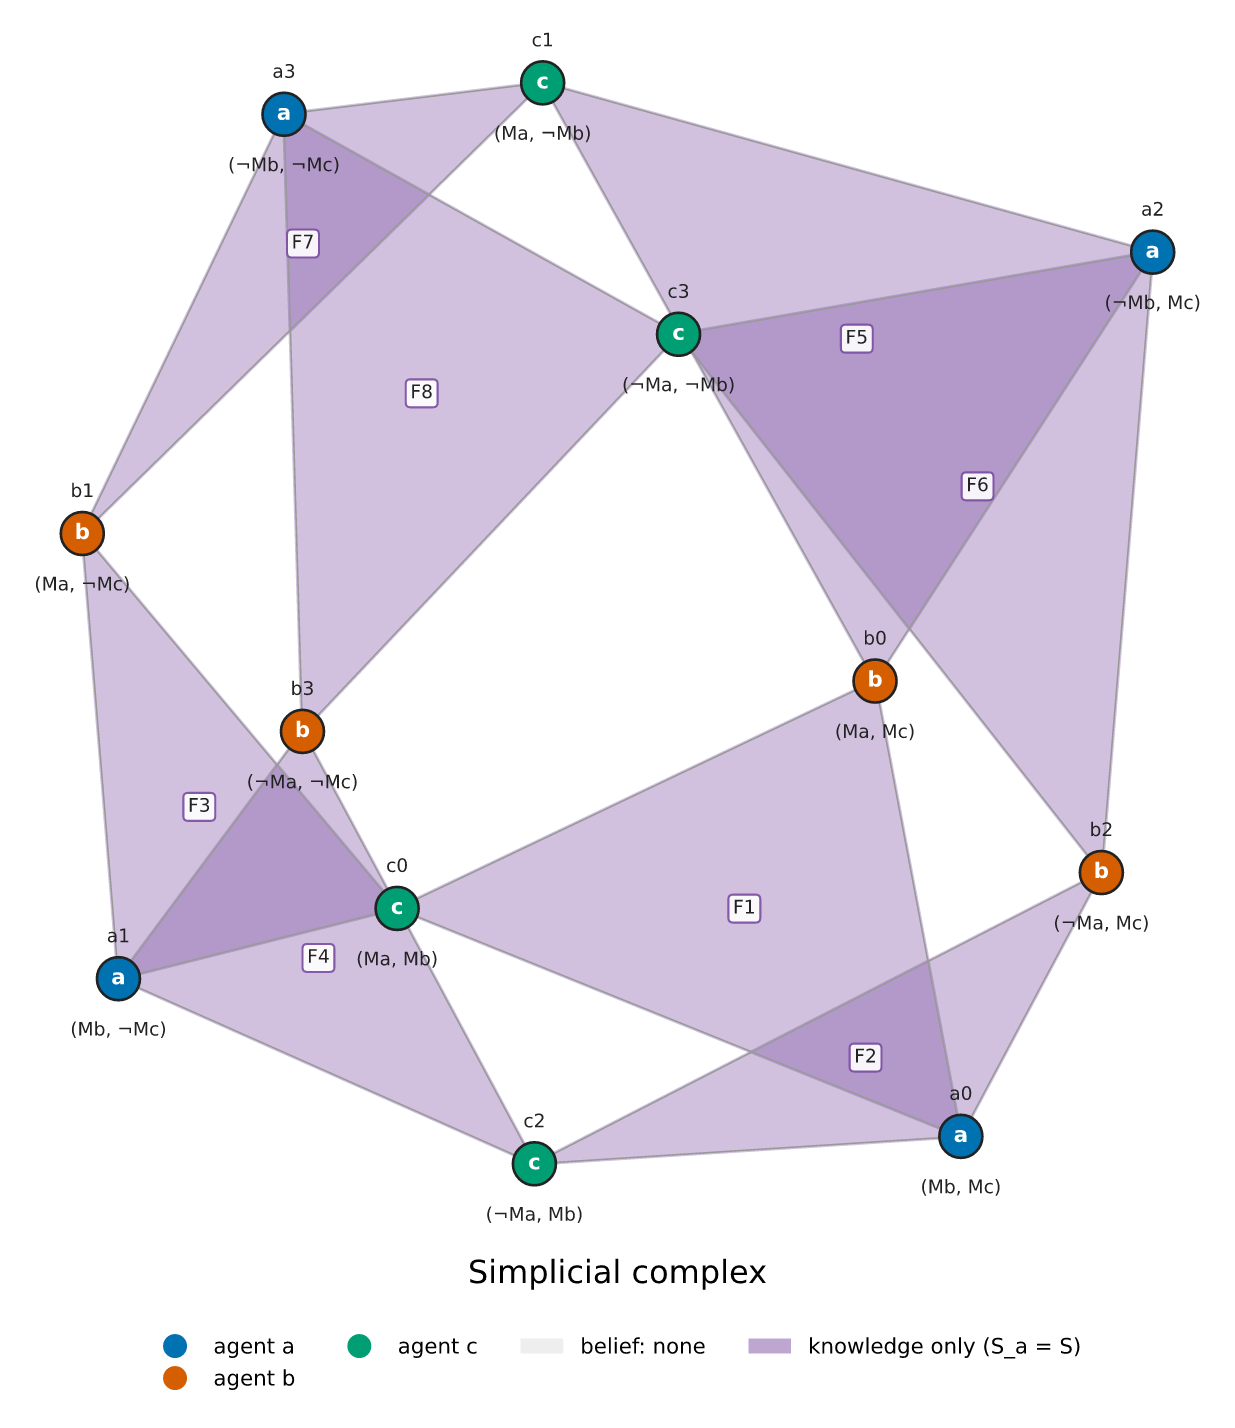
\includegraphics[scale=.12]{MuddyChildren.png}
\end{center}
		
		The simple explanation for what this project is/has done is implement the definitions from my thesis in an environment like Python
	\end{frame}

	\begin{frame}[fragile]
		\frametitle{Why Simulations?}
		\begin{center}
			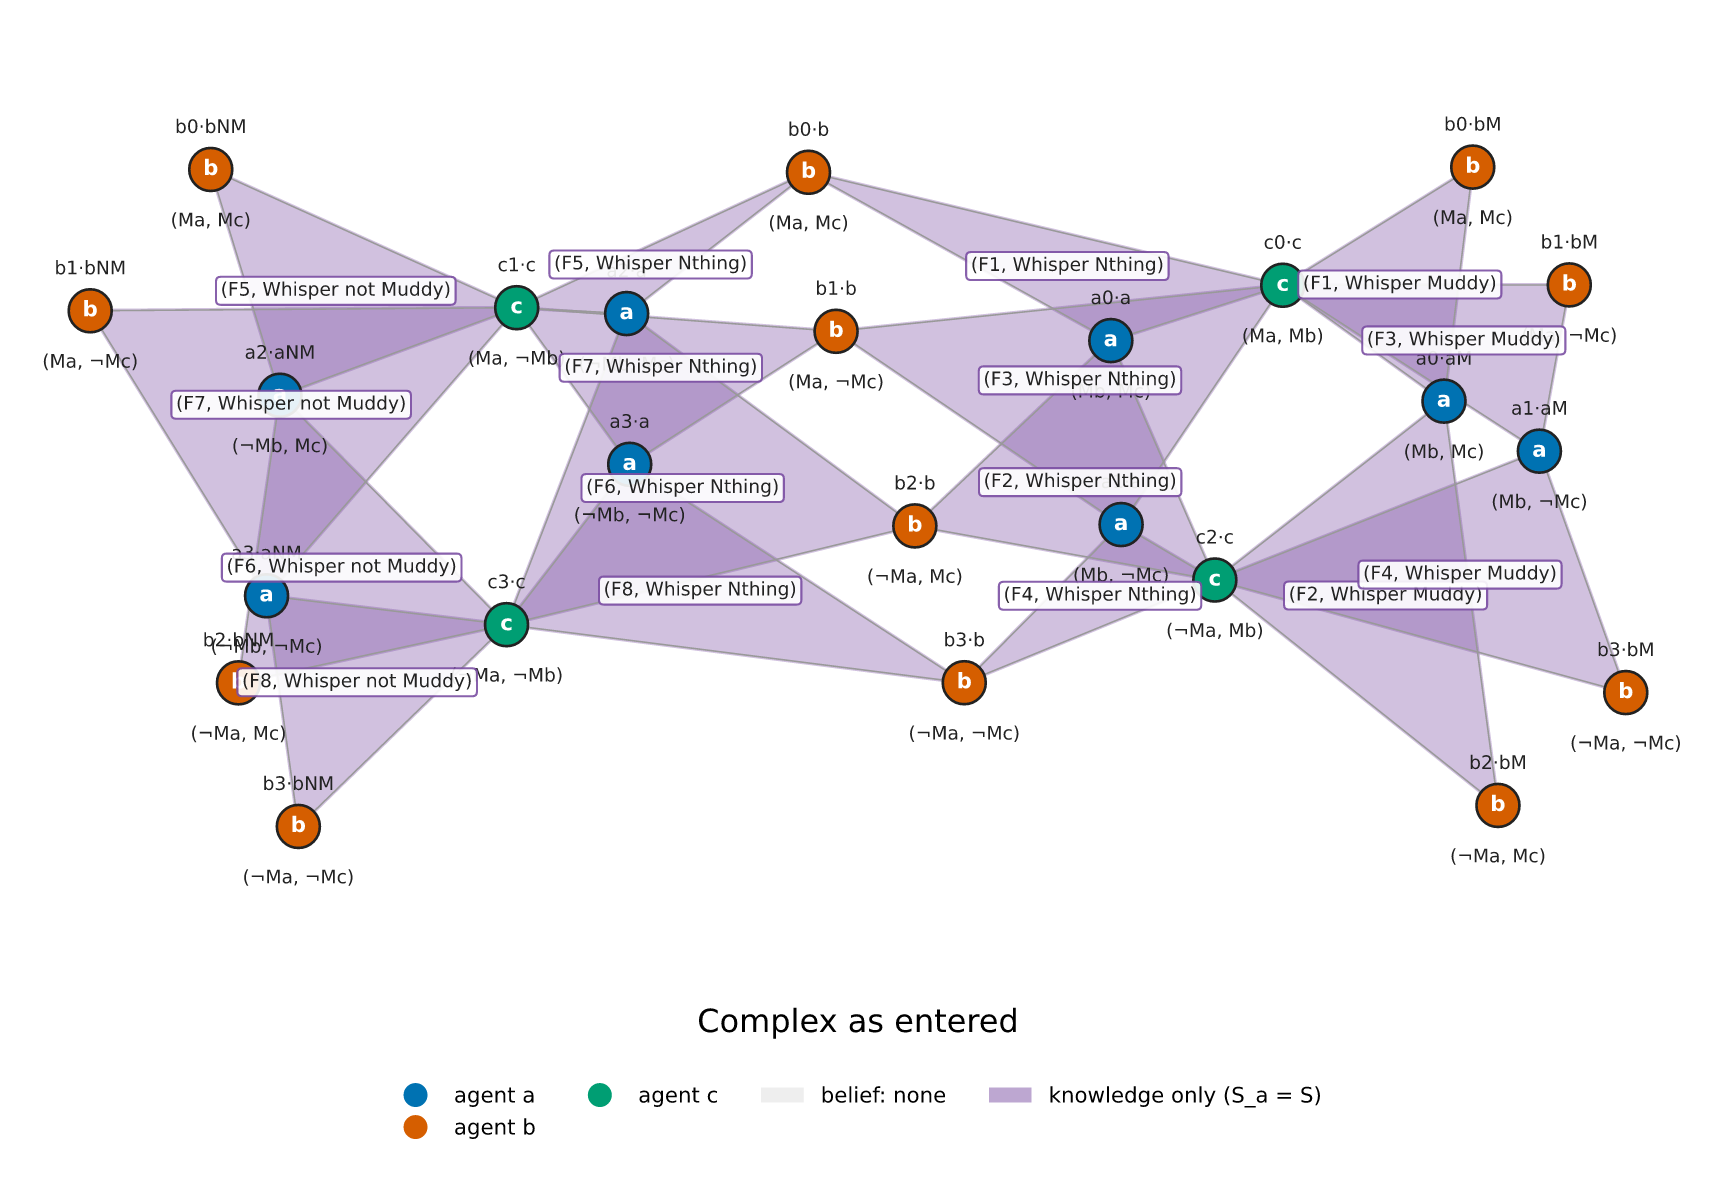
\includegraphics[scale=.11]{MCWhisper.png}
		\end{center}
		
		I believe there are two audiences for simulations of D.E.L. as we are undertaking\bigskip\pause
		
		The first is computer scientists: Insofar as D.E.L. is a language for describing distributed protocols\cite{SimpDEL,KaSC,KaG,ActionDC,CPM,CPaAM}, there is reason to simulate D.E.L. in order to simulate said protocols. \bigskip
	\end{frame}

		\begin{frame}[fragile]
		\frametitle{Why Philosophers?}
		\begin{center}
			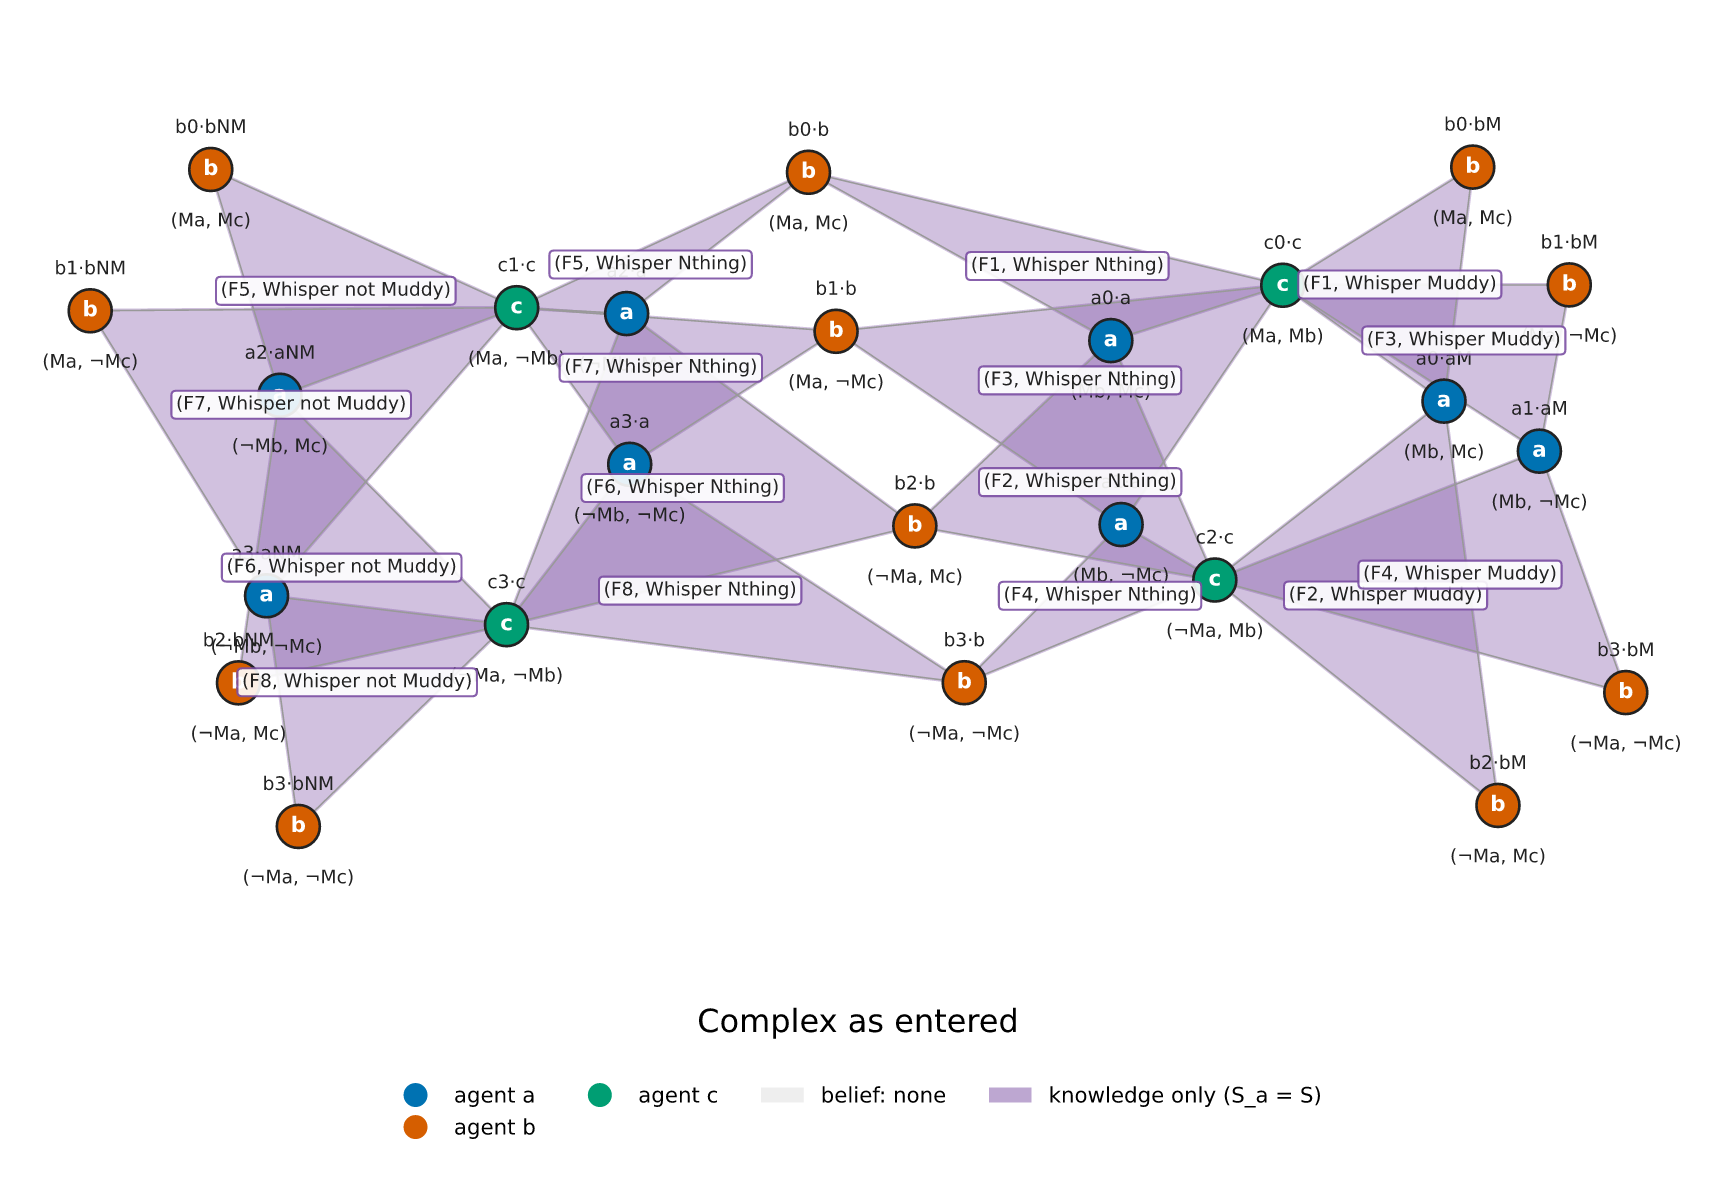
\includegraphics[scale=.06]{MCWhisper.png}
		\end{center}
		
	There are epistemic questions I think a framework like this might be able to tackle in a novel way.\bigskip\pause
		
		For example: ``Is Pluralistic Ignorance the kind of initial configuration belief revision is ideal for breaking''. \bigskip\pause
		
		Addressing this question would require a tool where one can compare the same ``scenario'' with revision switched on in one case and off in another.\bigskip\pause
		
		My ask: Can this setup address this meaningfully? What pitfalls should I expect? What other questions might this framework address (not necessarily involving revision)?
	\end{frame}
	

	\section{D.E.L. Simplicially}
	
	\subsection{What is Simplicial Semantics?}
	
	\begin{frame}[fragile]
		\frametitle{What is a Simplicial Model?}
		The foundational object in a simplicial (or local) model is a ``perspective''.\bigskip\pause
		
		Fixing a particular agent, a perspective for that agent consists of the most immediately ``available'' information for that agent.\bigskip\pause
		
		Given an agent $a\in Ag$, an $a$-perspective (or $a$-colored perspective) is an incomplete set of literals in some propositional language.\bigskip\pause
		
		An important point of contrast is a possible world, which is typically modeled as a complete set of literals.
	\end{frame}

	\begin{frame}[fragile]
	\frametitle{Example: Muddy Children Part 1}
				\begin{center}
			
\includegraphics[scale=.4]{muddychildrenimage.png}
		\end{center}
	
		Imagine you are the parent of three children, $a$, $b$, and $c$. You are a good parent, so these children are perfect reasoners.\bigskip\pause
		
		After playing outside $m>0$-many of the children are muddy.\bigskip\pause
		
		You sit the children in a circle. They can therefore observe the muddy status of every other child, but of course not themselves.
	\end{frame}



		\begin{frame}[fragile]
		\frametitle{Example: Muddy Children Part 1}
		The atomic facts in this example are $M_i$ for each child $i$: That is, the fact that is true iff $i$ is muddy. Literals are just atomic facts and their negations.\bigskip\pause
		
		Imagine being child $a$. Your perspective consists of all the facts corresponding to the muddiness of every child other than yourself. \bigskip\pause
		
		Your perspective consists of the muddy status of $b$ and $c$.\bigskip\pause
		
		Hence, simple combinatorial reasoning tells us there are four possible perspectives for each child.
	\end{frame}

	\begin{frame}[fragile]
		\frametitle{Uncertainty in Simplicial Semantics}
		We now need to model the fact that each child is uncertain about whether or not they themselves are muddy.\bigskip\pause
		
		Typically, uncertainty is modeled as an agent being unable to differentiate between distinct possibilities, or ``possible worlds''.\bigskip\pause
		
		When thinking perspectivally, or ``locally'', a possible world is a set of perspectives, one for each agent.\footnote{\tiny This assumption has some negative consequences I can discuss in much more detail during the Q\&A. The long story short is that no atomic fact can bet true without some agent knowing or believing it.}\bigskip\pause
		
		The idea behind uncertainty is then very simple. Suppose two sets of perspectives have a nonempty intersection.\bigskip\pause
		
		Agents whose perspectives are in this intersection \textit{have the same perspective} in these sets. Hence, they cannot tell them apart, and are uncertain between these two sets.
	\end{frame}



	\begin{frame}[fragile]
		\frametitle{Example: Muddy Children Part 2}
		The question is then which sets of perspectives are valid ``sets'' \bigskip\pause
		
		Placing yourself in $a$'s perspective, the question is, which of $b$ and $c$'s perspectives do you consider possible simultaneously?\bigskip\pause
		
		The answer (for this example) is fortunately simple: They're seeing information consistent with yours, plus they have to \textit{agree} as to whether or not you are muddy.\bigskip\pause
		
		This corresponds, in this setup, to all consistent \textit{uniquely colored} sets, e.g., those with exactly one perspective per agent.
	\end{frame}

	\begin{frame}[fragile]
	\frametitle{Example: Muddy Children Part 2}
	\begin{center}
		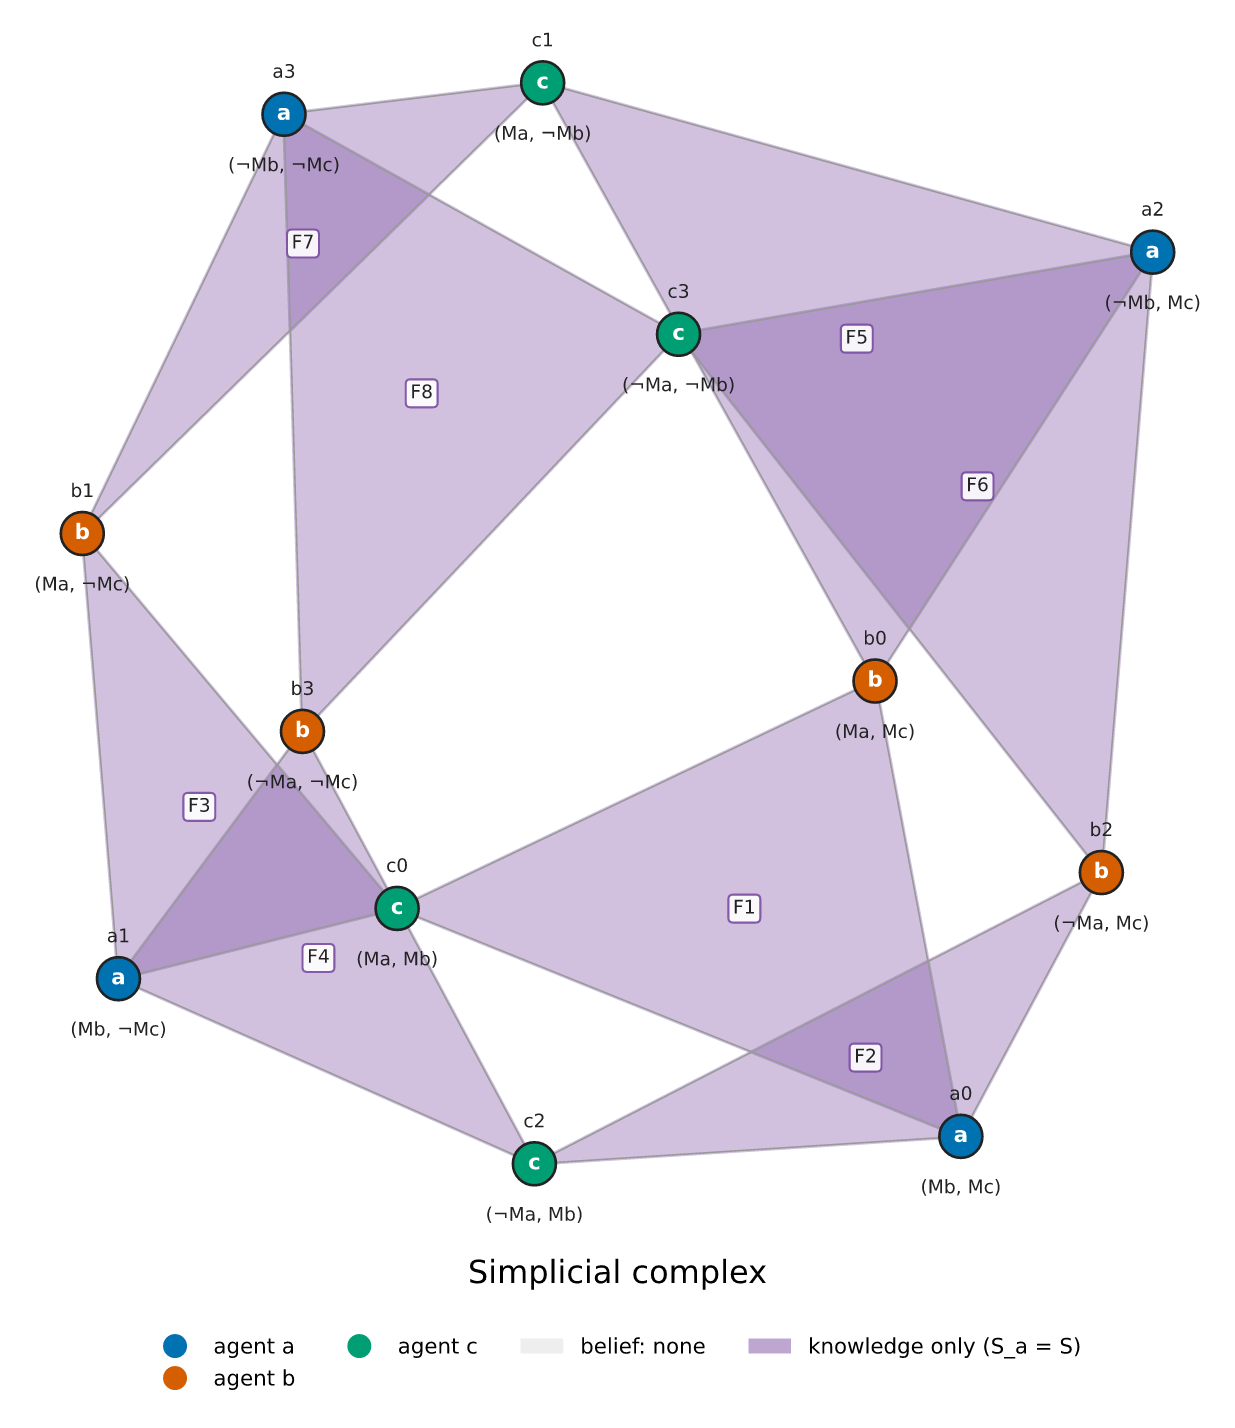
\includegraphics[scale=.16]{MuddyChildren.png}
	\end{center}
\end{frame}

	\subsection{What is D.E.L.?}
	
	\begin{frame}[fragile]
		\frametitle{Dynamics}
		Imagine you, the parent, stands in the center of the circle of children, and announce that ``some of you have mud on your forehead''.\bigskip\pause
		
		How should the children respond to this info?\bigskip\pause
		
		Intuitively, this announcement correspond to each child learning $M_a\vee M_b\vee M_c$, learning every other child learns this fact, and so on.\bigskip
		
		We represent that with ``update perspectives'' as follows, and call this an \textit{action}.
	\end{frame}

	\begin{frame}[fragile]
		\frametitle{Public Announcement Update}
		In particular, this action is a ``public announcement'': there is one perspective per agent, and every agent considers that perspective correct in the update.\bigskip\pause
		
		The idea with actions is that they can be combined with inputs to give outputs using a restriction of the Cartesian product.\bigskip\pause
		
		What's true at a perspective in an action is what \textbf{has} to be not false\footnote{\tiny This is not the only interpretation possible. Indeed, one could force entailment, not just consistency} in an input perspective for this action to apply/change it. This is called a \textit{precondition}.
	\end{frame}

	\begin{frame}[fragile]
	\frametitle{Public Announcement Update}

	\begin{center}
		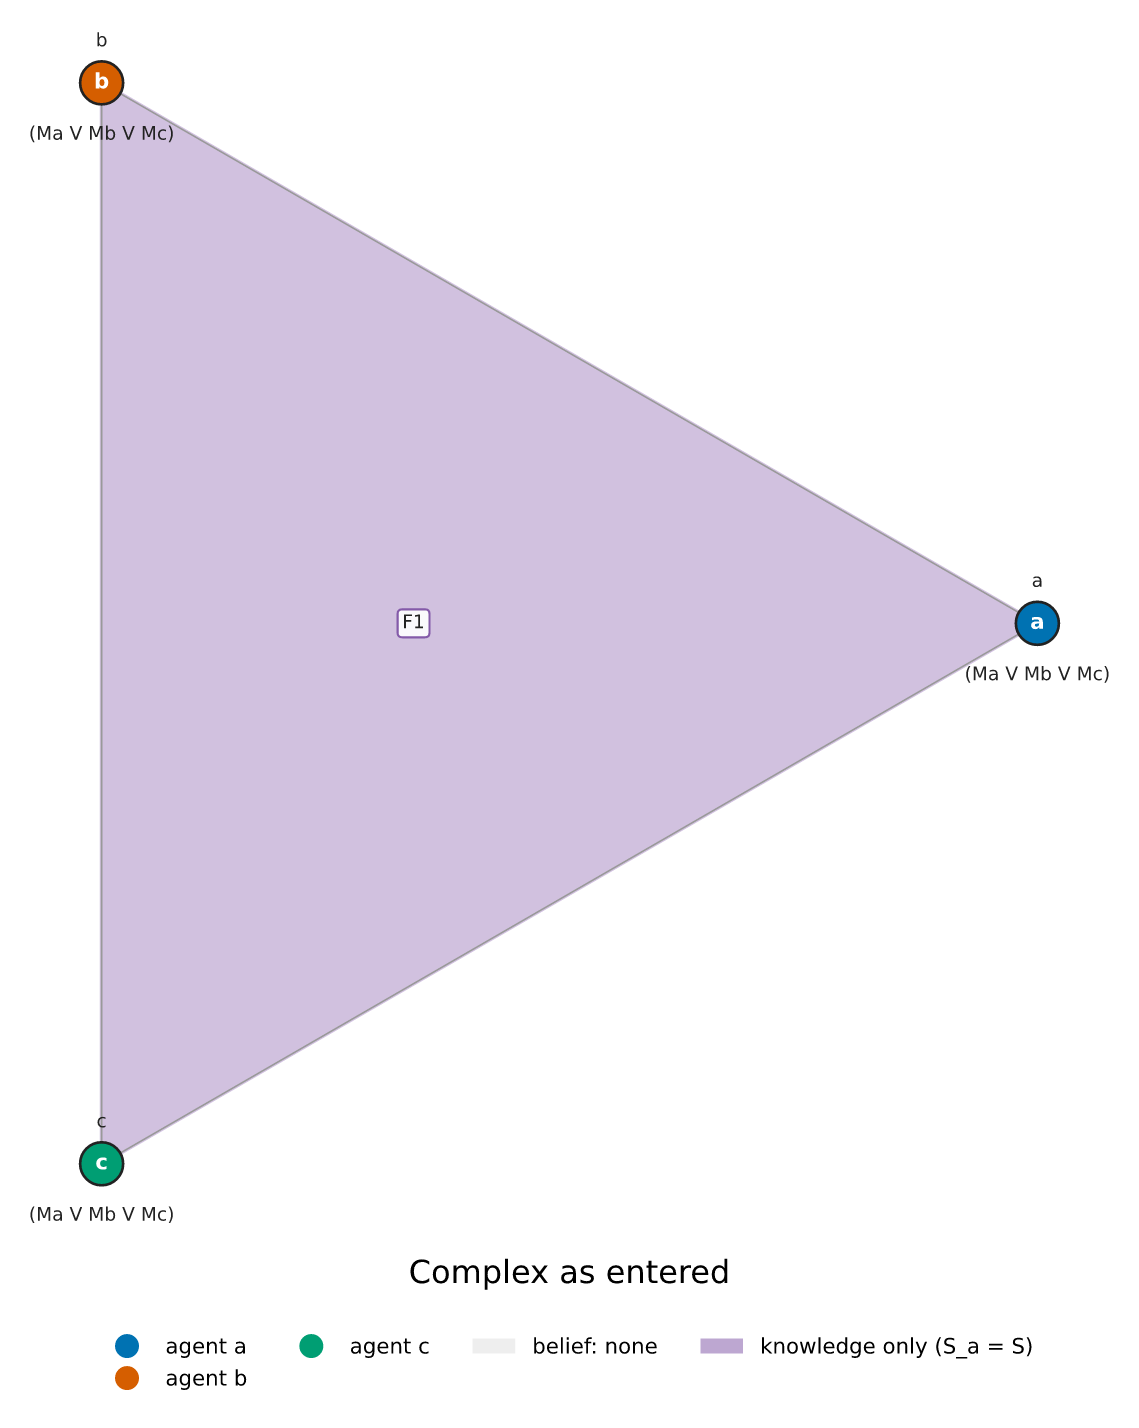
\includegraphics[scale=.12]{PA.png}
	\end{center}

\end{frame}

\begin{frame}[fragile]
	\frametitle{Public Announcement Update}
	If we match preconditions to the input, and draw facets when the first and second projections appear in both the input and action respectively, we get the following output.
	
	\begin{center}
		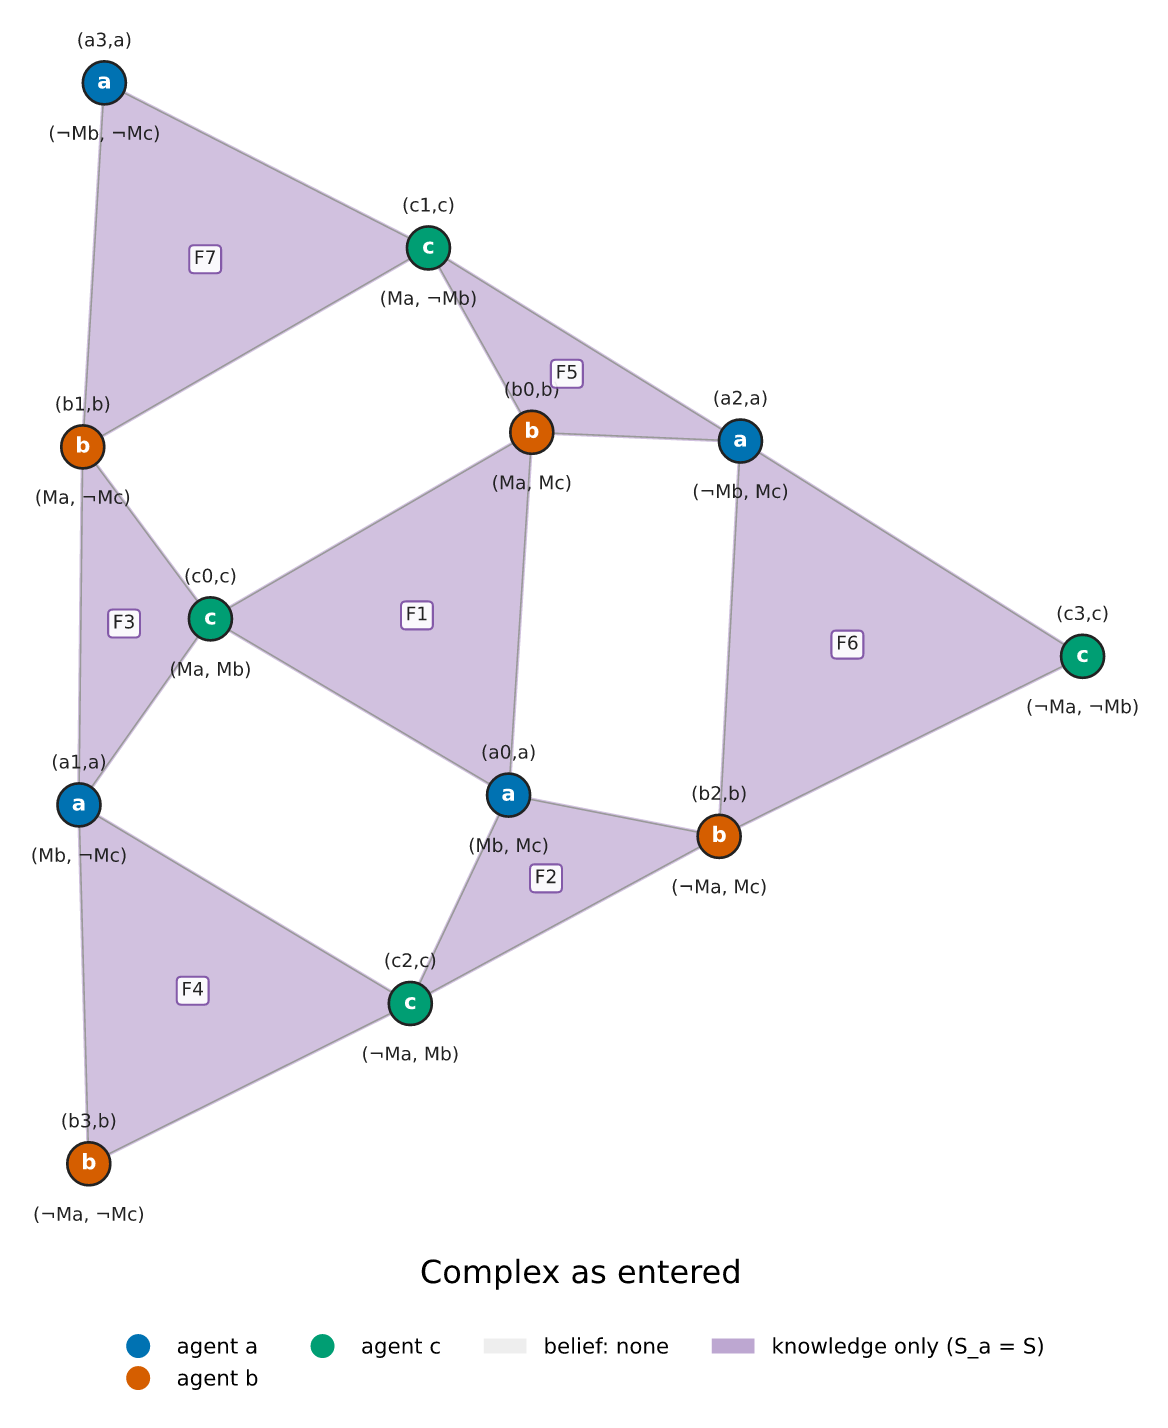
\includegraphics[scale=.13]{MuddyAfterPA.png}
	\end{center}
\end{frame}

	\begin{frame}[fragile]
		\frametitle{Subtler actions}
		Suppose $a$ whispers something to $b$. $c$ observes this, and knows that $a$ is not a liar.\bigskip\pause
		
		What does this action look like?
		
		\begin{center}
			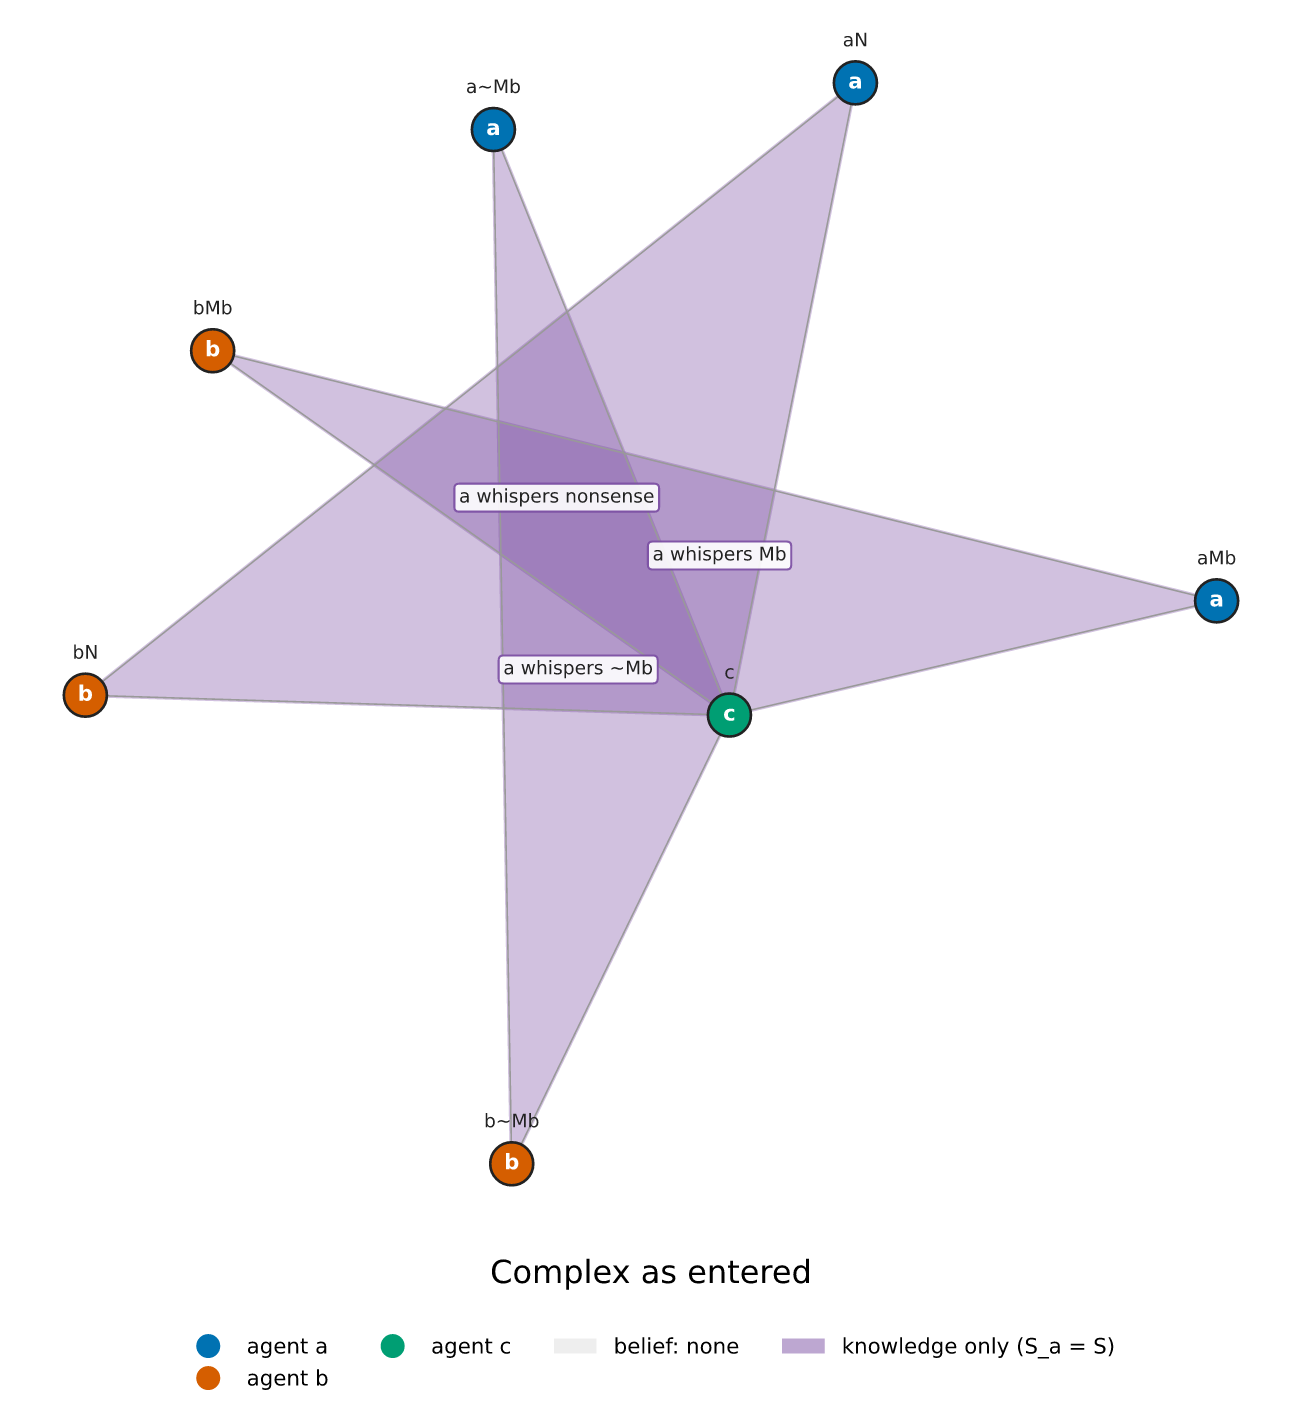
\includegraphics[scale=.12]{Whispering.png}
		\end{center}
	\end{frame}

	\begin{frame}[fragile]
		\frametitle{Subtler Update}
	Now let's apply this action to the same input.
	
	\begin{center}
		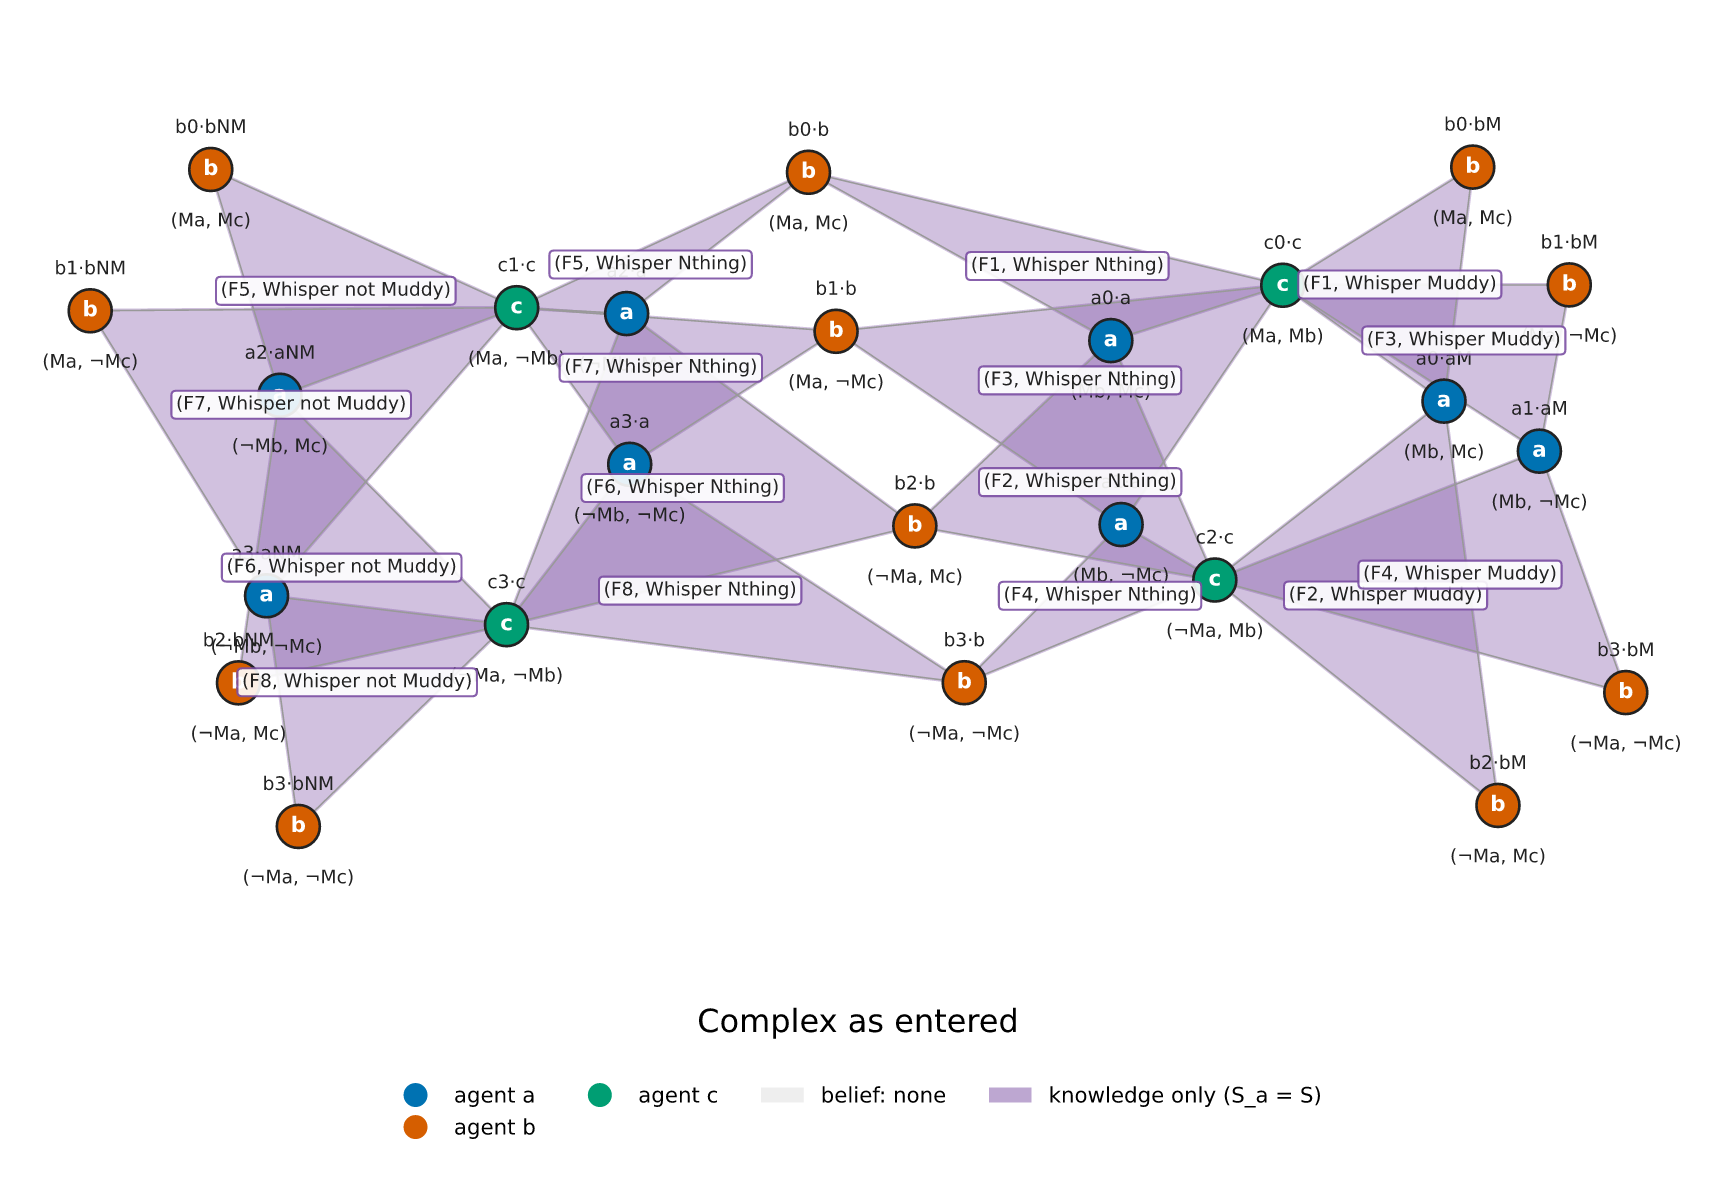
\includegraphics[scale=.17]{MCWhisper.png}
	\end{center}
	\end{frame}
	
	\subsection{Revision Under Simplicial D.E.L.}
	
	\begin{frame}[fragile]
		\frametitle{False Beliefs}
	So far, the children are perfect reasoners and have no misconceptions. What if that were not the case?\bigskip\pause
	
	Of all the sets of perspectives, some children may only consider some sets possible. Indeed, they not not consider the ``true'' set possible!\bigskip\pause
	
	As such, some sets of perspectives will only ``belong'' or be ``assigned'' to a portion of all the agents. Agents only consider worlds ``belonging'' or ``assigned'' to them possible.\bigskip\pause
	
	So, agents are less uncertain, but potentially incorrect!
	\end{frame}

	\begin{frame}[fragile]
		\frametitle{Actions with False Beliefs}
		Now imagine $c$ doesn't observe that $a$ is whispering to $b$. $a$ and $b$ believe that $c$ is not observing them, either.\pause
		
	\begin{center}
		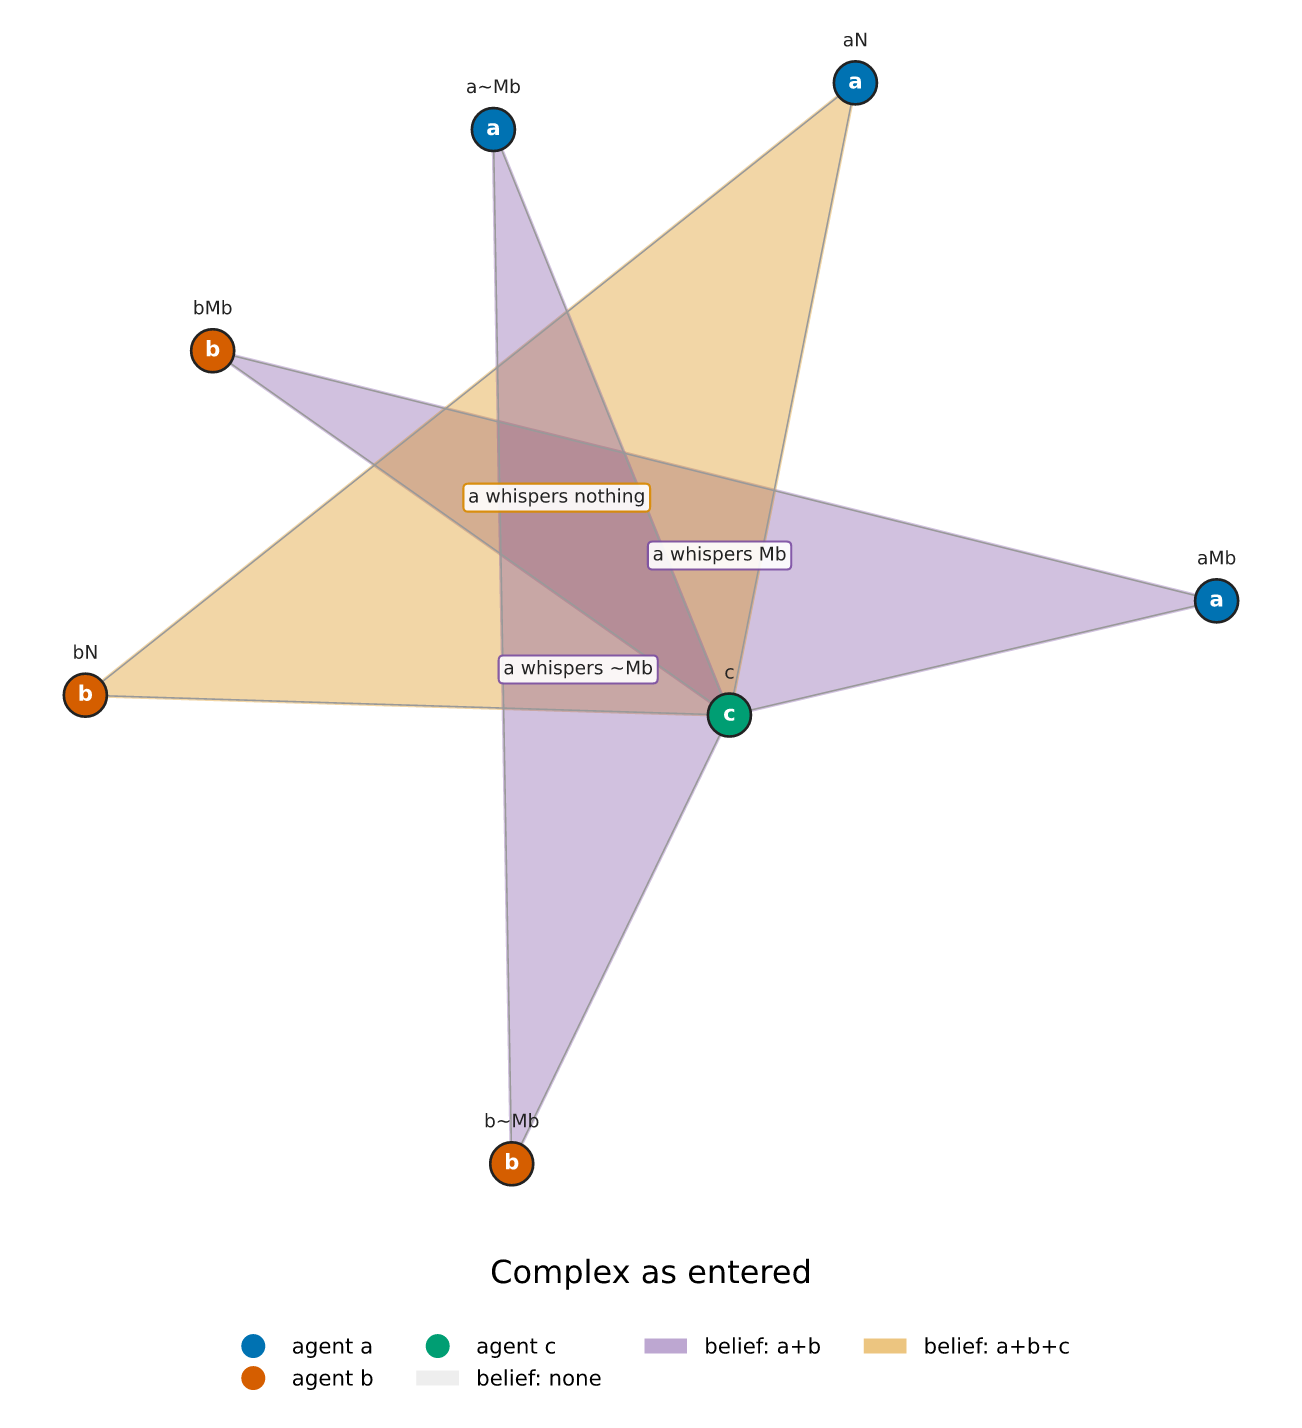
\includegraphics[scale=.1]{Whisper False.png}
	\end{center}
	
	Observe: $c$ has false beliefs in this action.
		
	\end{frame}

	\begin{frame}[fragile]
		\frametitle{False Belief Update}
		By matching perspectives using preconditions, and drawing facets present in both the input from before and this new action we can again compute the output.\pause
		
		\begin{center}
			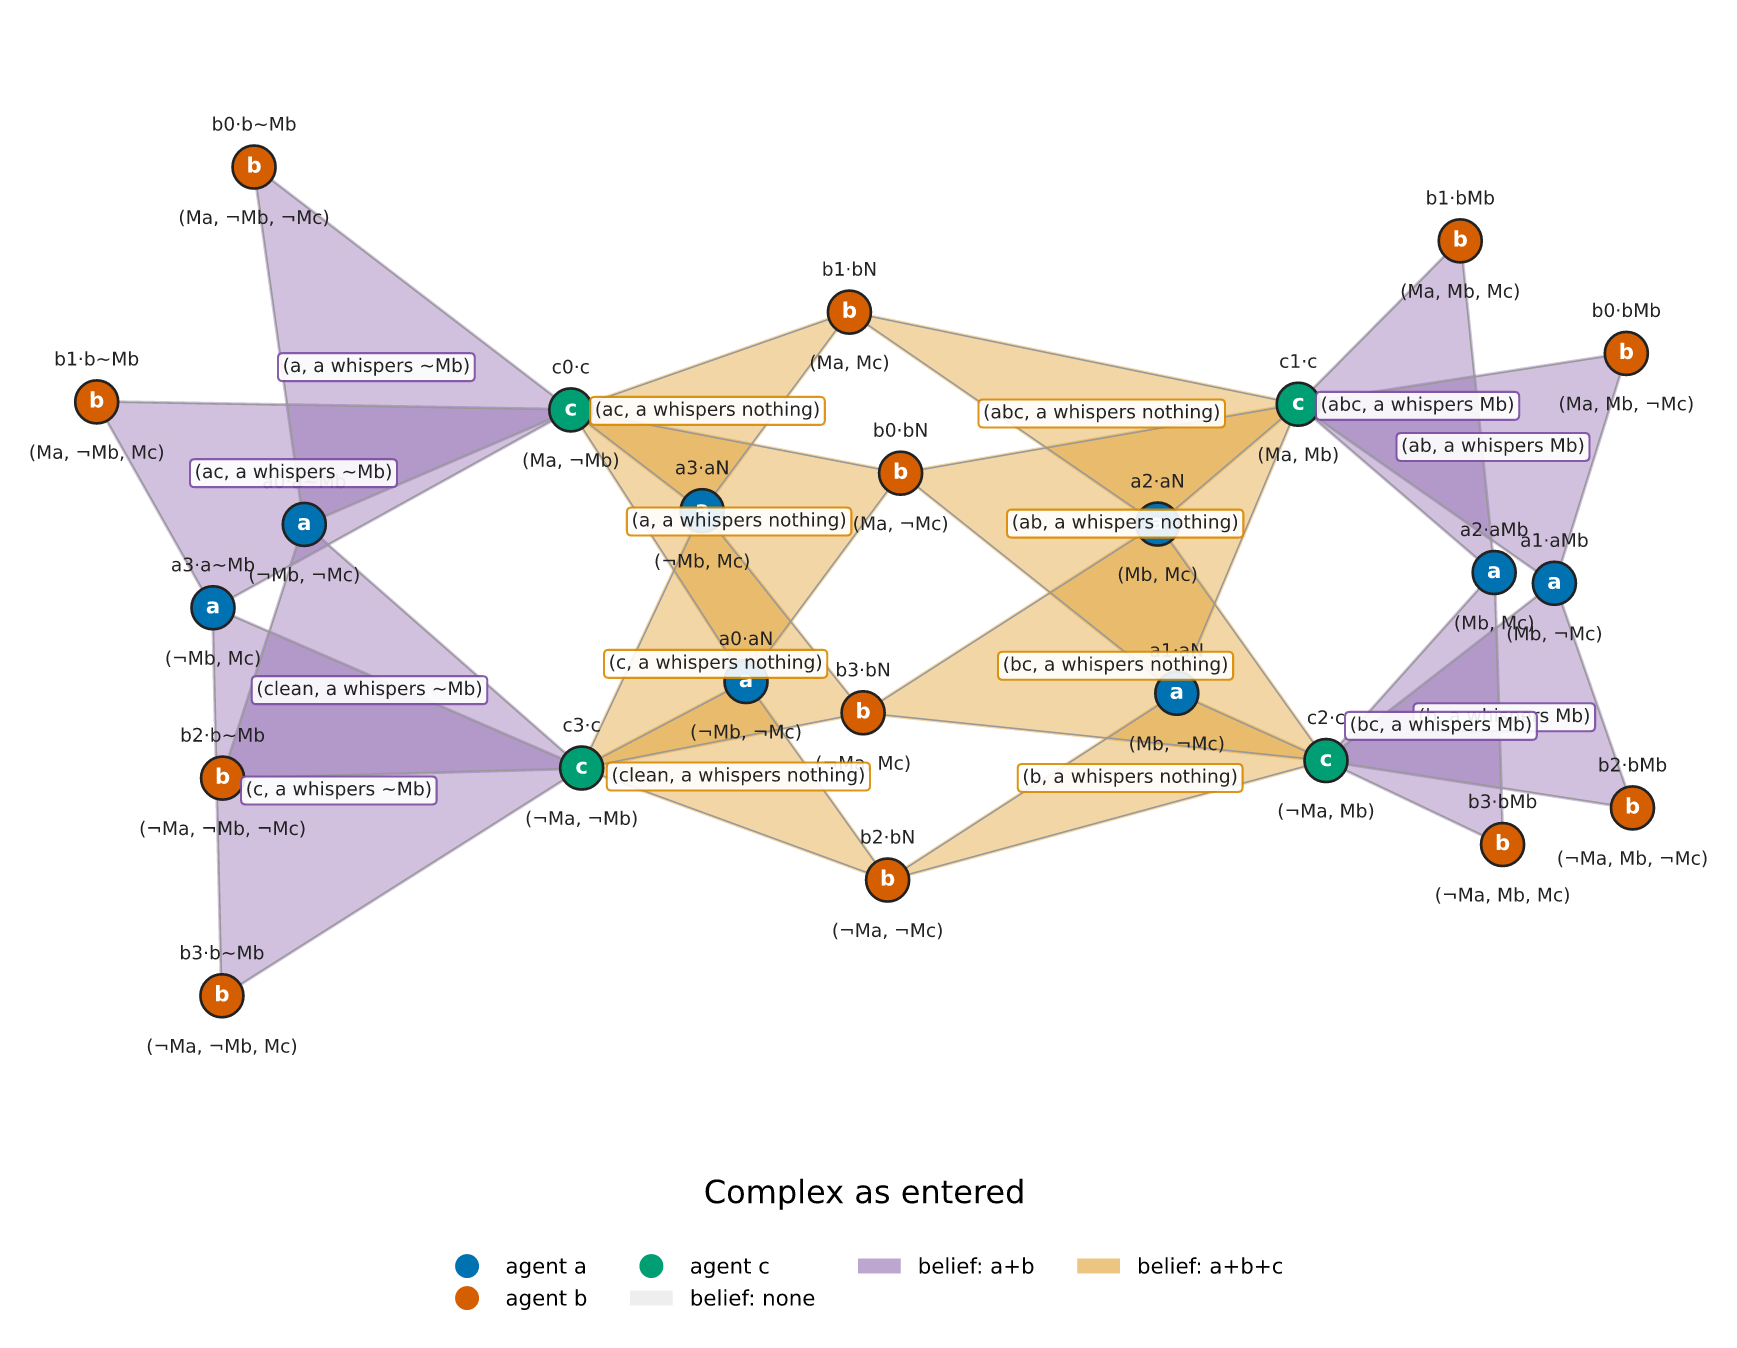
\includegraphics[scale=.11]{MCFWhisperN.png}
		\end{center}
		
		Observe: Despite not having false beliefs in the input, $c$ has false beliefs in the output.
	\end{frame}

	\begin{frame}[fragile]
		\frametitle{Actions with Revision}
		Now imagine you as the parent publicly call $a$ out for whispering to $b$. So, it's common knowledge now that $a$ said something. Again, let's assume $a$ told $b$ her muddy status.\bigskip\pause
		
		We already know what a public announcement looks like:
		
		\begin{center}
			\includegraphics[scale=.11]{PAWhisper.png}
		\end{center}

	\end{frame}

		\begin{frame}[fragile]
		\frametitle{Actions with Revision}
		And we can compute the output:
		
		\begin{center}
			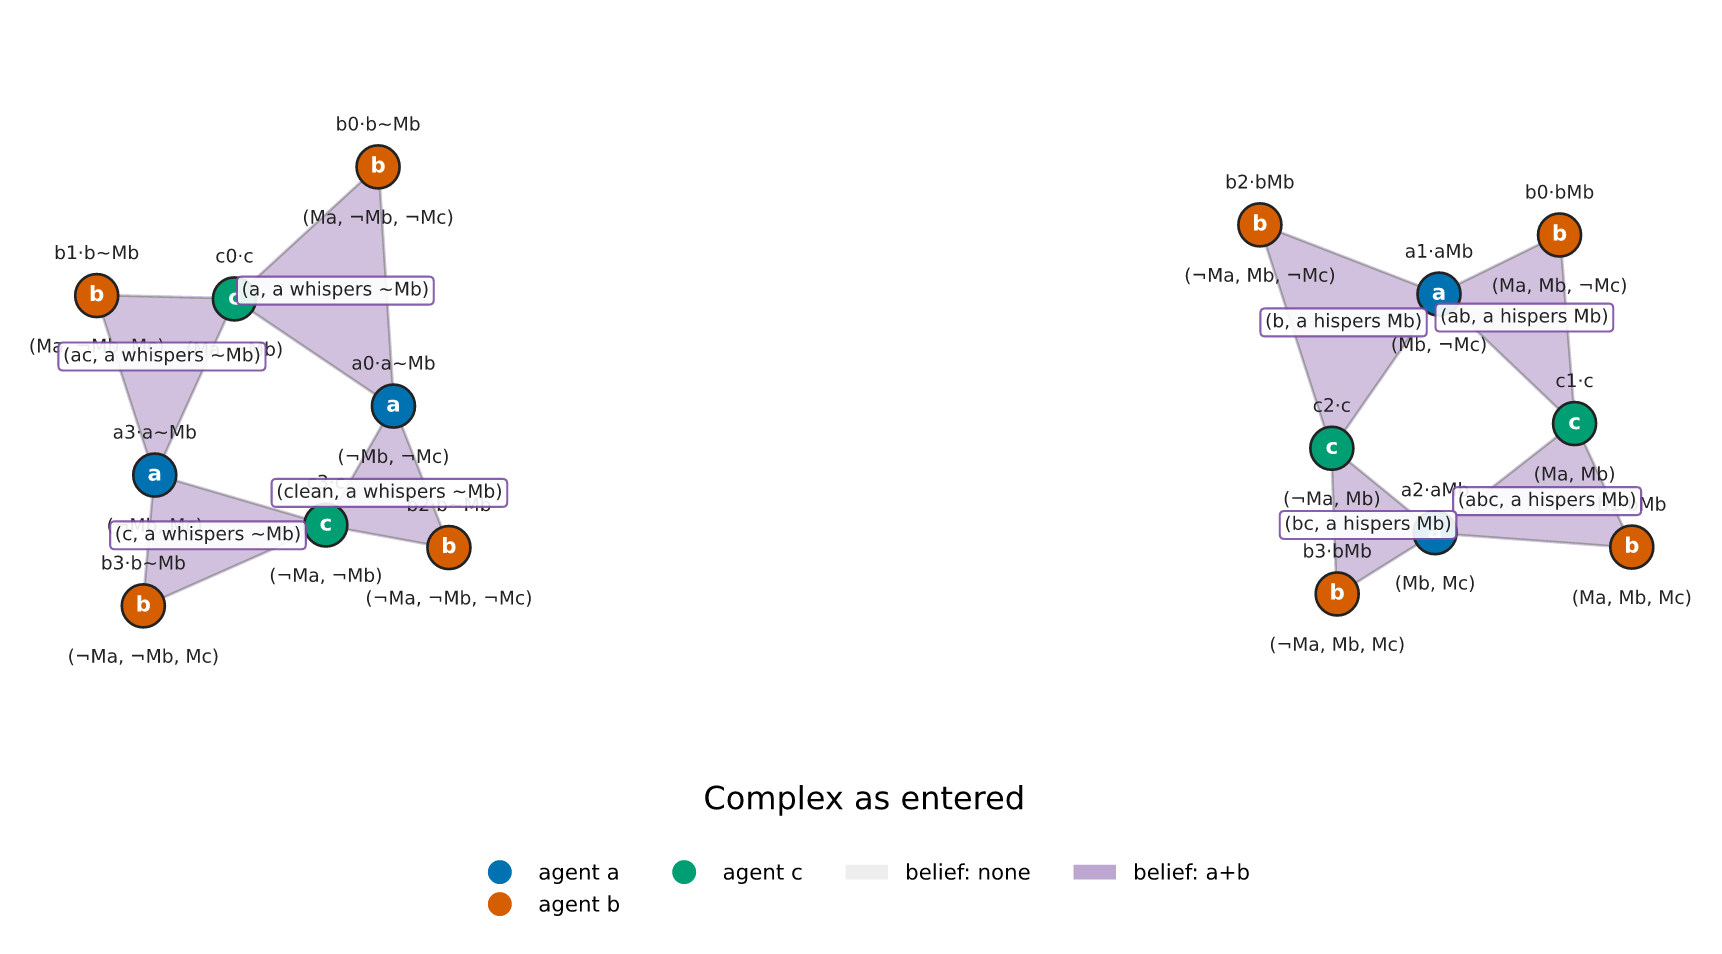
\includegraphics[scale=.16]{MCAfterWhisperPA.png}
		\end{center}
		
		Observe: $c$ doesn't just have false beliefs, she believes nothing (or, equivalently, anything)!
		
		
		
		
	\end{frame}

	\begin{frame}[fragile]
		\frametitle{Actions with Revision}
		If we compute the update differently, we can allow $c$ to learn in a subtler way.\begin{center}
			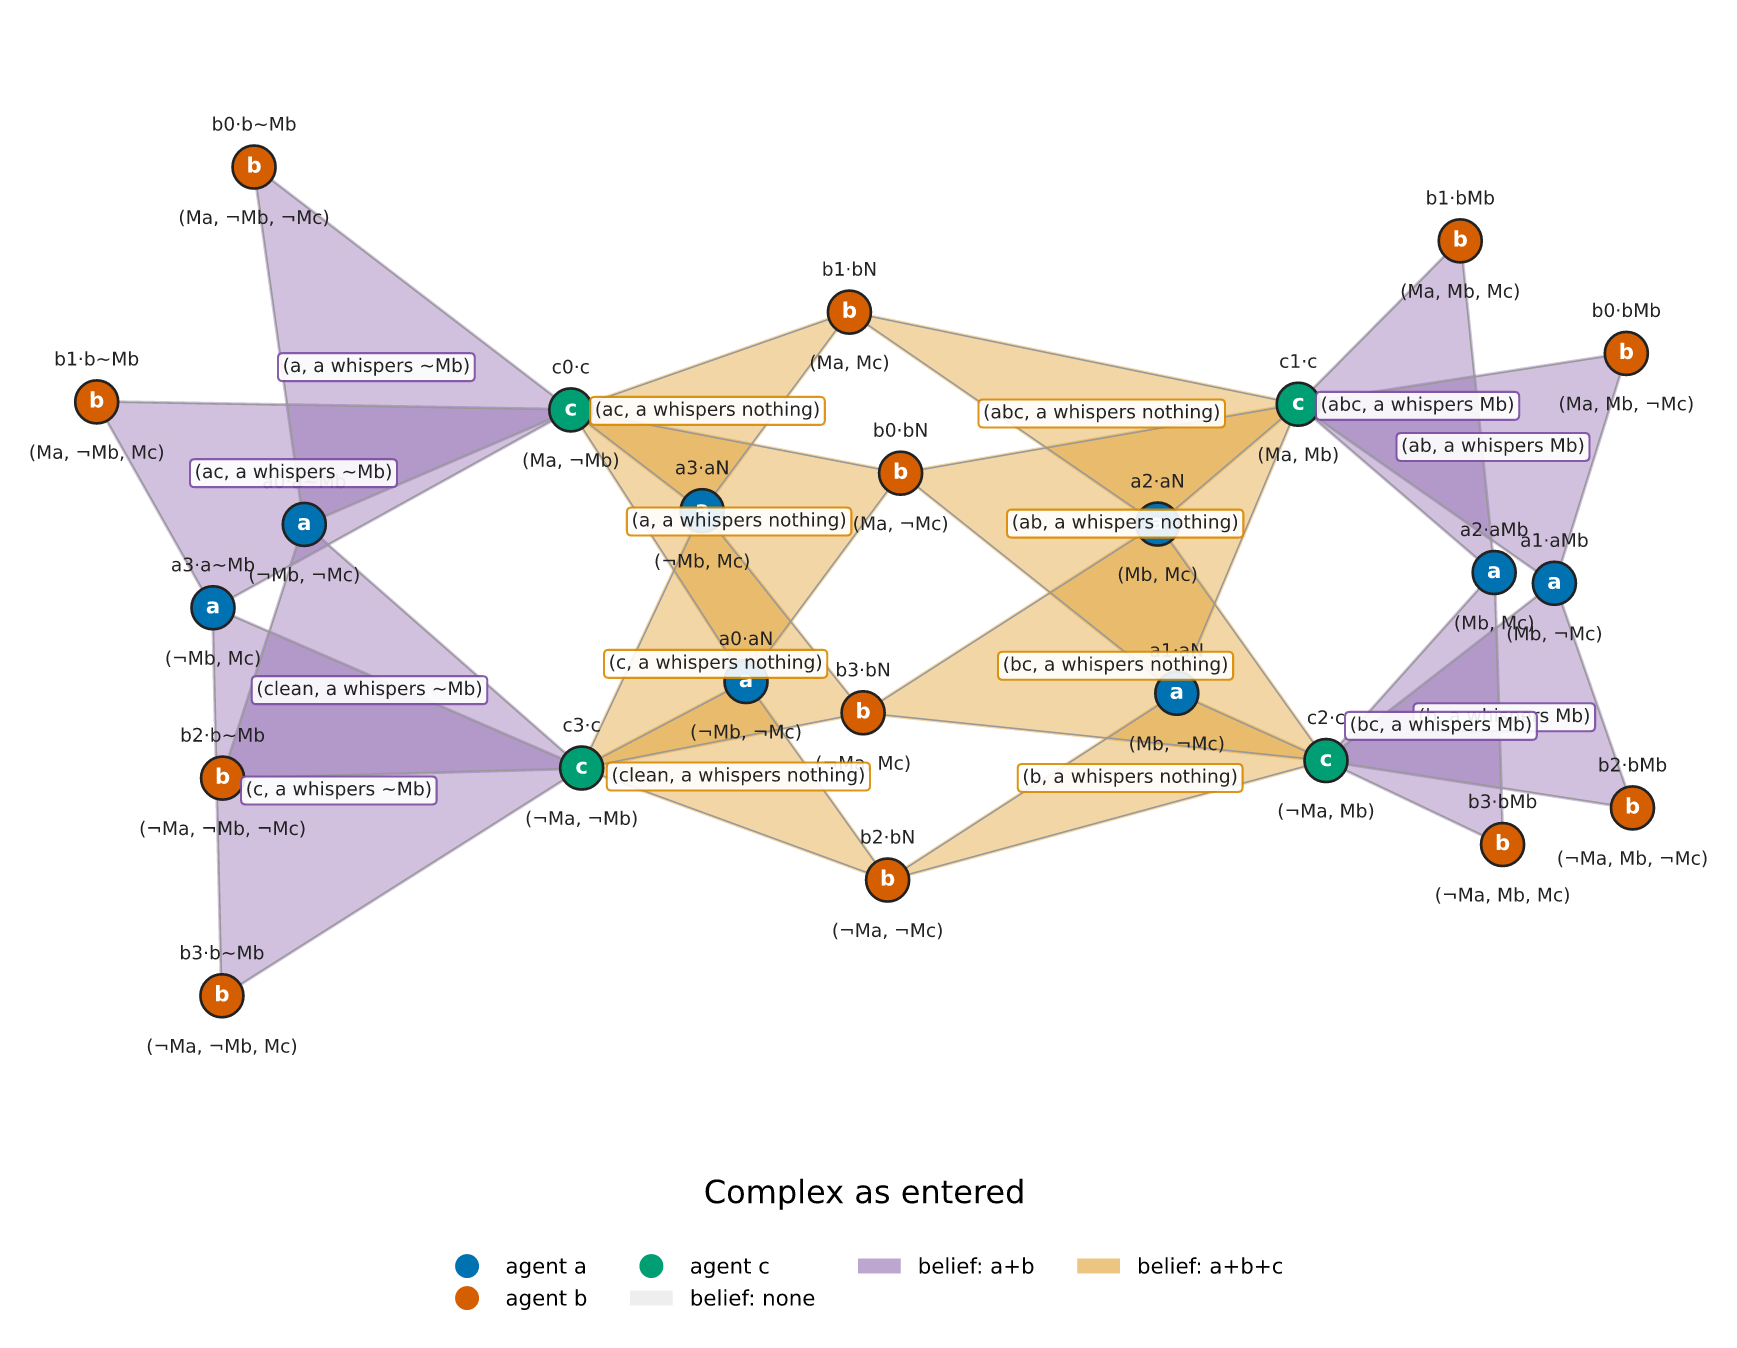
\includegraphics[scale=.1]{MCFWhisperN.png}
		\end{center}
		
		$c$ can ``replace'' lost sets with ``similar'' ones.\cite{Lewis2,Stalnaker1981,AGM}\bigskip\pause
		
		One metric for ``similarity'' is to say that two sets are more similar if they share more perspectives in common. 
	\end{frame}

	\begin{frame}[fragile]
		\frametitle{Actions with Revision}
		This computation is a (lot) more complicated in general. But, it gives the following output.
		
		\begin{center}
			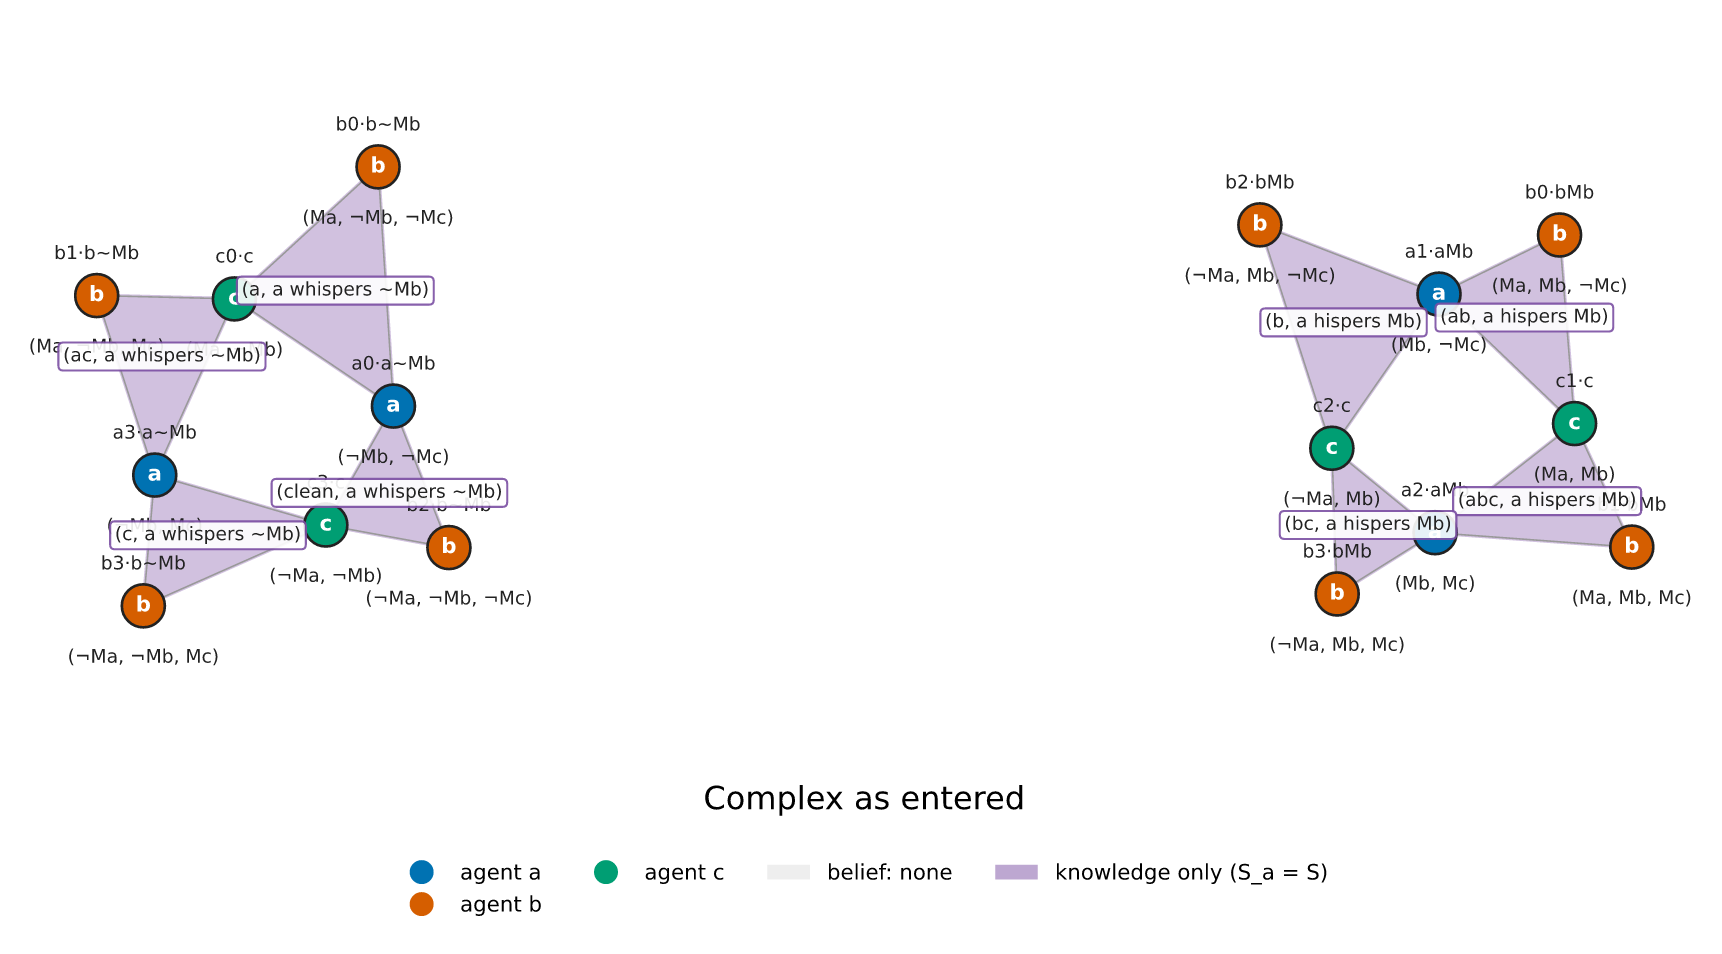
\includegraphics[scale=.17]{MCRevision.png}
		\end{center}
	\end{frame}
	
	\section{Live Demo}
	
	\section{Goals For Simulations}
	
	\begin{frame}[fragile]
		\frametitle{Future Questions}
			The hope is that by using this tool we can compute larger examples more quickly, and make more comparisons more easily.\bigskip\pause
			
			This would let us test questions such as:
			\begin{itemize}
				\item Can we categorize initial configurations for which an agent that learns by revision tends to perform better?\pause
				\item Can we identify protocols that perform better, under some specified metric, when the agent learns via revision instead of classically?\pause
				\item How does revision affect or change many existing, traditional protocols?\pause
				\item Comparing the same protocol across different initial configurations, can we find protocols which don't succeed \textit{always} but do well \textit{typically}? Could this be a defense for some known but generally discarded protocols?
			\end{itemize}
	\end{frame}

	\begin{frame}[fragile]
	\frametitle{Future Questions}
	\begin{center}
		\includegraphics[scale=.7]{Drinking.jpg}
	\end{center}
	Consider Pluralistic Ignorance (where everyone has a belief that $P$ but a false belief that everyone else believes $\neg P$)\bigskip\pause
	
	Modeling Pluralistic Ignorance in epistemic logic isn't new.\cite{Christoff}\bigskip\pause
	
	Would revision help avoid entering Pluralistic Ignorance? (prediction, no)\bigskip\pause
	
	Would revision help in leaving Pluralistic Ignorance? (prediction, yes)
\end{frame}


	
	%---------------------------------------------------------
	
	\begin{frame}[fragile]
		\begin{center}
		Thank You!
		\end{center}
		
	\end{frame}

	\section{Sources}
	
	\begin{frame}[allowframebreaks]{Sources}
		\printbibliography
	\end{frame}
	
	%---------------------------------------------------------
	
	\section*{Detail Slides}
	
		\begin{frame}[fragile]
		\frametitle{Disadvantages}
		\begin{itemize}
			\item The following are sound for any $P\in\mathfrak{P}$:
			$$\mathbf{NU_K}:P\rightarrow\bigvee_{a\in Ag}K_aP$$
			$$\mathbf{NU_B}:P\rightarrow\bigvee_{a\in Ag}B_aP$$
			\item This is because we chose to assign atoms to nodes, rather than facets
			\item However, \textbf{NU} is slightly more general than similar formulas in the literature \cite{KaSC}
		\end{itemize}
	\end{frame}
	
	\begin{frame}[fragile]
		\frametitle{Comparison with Previous Work}
		\begin{itemize}
			\item Semantics for belief in simplicial complexes has been tried twice before \cite{KaSC,SimpBel}
			\item Our approach has some clear advantages, however.
			\item In \cite{KaSC}, the axiom $K_a\varphi\rightarrow B_a\varphi$ is not sound
			\item If one restricts to models where this is sound, the stronger statement $K_a\varphi\leftrightarrow B_a\varphi$ becomes sound
			\item In \cite{SimpBel}, the models are not UCF
			\item If one restricts to UCF models, $K_a\varphi\leftrightarrow B_a\varphi$ becomes sound
			\item Our system is the only simplicial semantics for belief we are aware of that is:
			\begin{itemize}
				\item UCF
				\item $K_a\varphi\rightarrow B_a\varphi$ is sound
				\item $K_a\varphi\leftrightarrow B_a\varphi$ is not sound
			\end{itemize}
		\end{itemize}
	\end{frame}
	
\begin{frame}[fragile]
	\frametitle{Simplicial Sets}
	\begin{itemize}
		\item It would be nice to avoid making axioms like \textbf{NU} sound
		\item There are many possible ways to do this, including ``environment'' nodes or hypergraphs \cite{HG}
		\item One promising avenue is to use ``simplicial sets'' as opposed to simplicial complexes
		\item This allows multiple faces to be drawn on the same set of vertices 
	\end{itemize}\begin{columns}
		\begin{column}{0.5\textwidth}
			\begin{center}
				\begin{tikzcd}[scale cd=.6]
					& w_0 \arrow[red, ldd] \arrow[red, rdd] \arrow[blue, ldd, bend right] \arrow[green6, rdd, bend left] &                                                                                                                  \\
					&                                                                            &                                                                                                                  \\
					w_1 \arrow[red, rr, leftrightarrow] \arrow[green6, rr, bend left] \arrow[red, loop, distance=2em, in=305, out=235] \arrow[blue, loop, distance=2em, in=215, out=145] &                                                                            & w_2 \arrow[blue, ll, bend left] \arrow[red, loop, distance=2em, in=305, out=235] \arrow[green6, loop, distance=2em, in=35, out=325]
				\end{tikzcd}
			\end{center}
		\end{column}
		\begin{column}{0.5\textwidth}
			\begin{center}
				\begin{tikzcd}[scale cd=.6]
					& \color{red}a_1 \arrow[ldd, no head] \arrow[purple6, ldd, no head, bend right] \arrow[orange, ldd, no head, bend right=49] &                                                                                                             \\
					&                                                                                                          &                                                                                                             \\
					\color{blue}b_1 \arrow[rr, no head] \arrow[purple6, rr, no head, bend right] \arrow[orange, rr, no head, bend right=49] &                                                                                                          & \color{green6}c_1 \arrow[luu, no head] \arrow[purple6, luu, no head, bend right] \arrow[orange, luu, no head, bend right=49]
				\end{tikzcd}
			\end{center}
		\end{column}
	\end{columns}
	
	
	
\end{frame}

\begin{frame}[fragile]
	\frametitle{Awareness}
	\begin{itemize}
		\item Key difference between simplicial models and Kripke models is that some formulas are ``assigned'' to an agent at a world/facet
		\item We could formalize this
		\item Let $A_i$ be a new modality for $i\in Ag$ which applies to literals
		\item $\M,X\vDash A_a P$ iff $L(\pi_a(X))(P)=1$
		\item Can read as ``a is aware of $P$'', similar to \cite{Awareness}
		\item Also motivates trying to get more complicated formulas (e.g., not literals) into perspectives
	\end{itemize}
	
\end{frame}

\begin{frame}[fragile]
	\frametitle{Belief Merging}
	\begin{itemize}
		
		\item The idea is still vague. But, there is an intuition that we can we can associate perspectives with belief sets
		
		\item Taking two perspectives (for different agents) could we use our notion of ``nearness'' to find a ``best way'' to combine them?
		\item Consider two perspectives $x$ and $y$, and Let $\mathcal{X}$ and $\mathcal{Y}$ be the set of facets containing $x$ and $y$ respectively
		
		\item If agents beliefs come from a set of facets $W$, traditional merging is $\mathcal{X}\cap\mathcal{Y}\cap W$
		
		\item Perhaps $X\in\mathcal{X}\cap W$ but $X\notin\mathcal{Y}$
		
		\item Yet, there is $X'\notin W$ such that $X'\in\mathcal{X}\cap\mathcal{Y}$ and $X$ and $X'$ are near.
		
		\item Perhaps $X'$ should be included in merging?
	\end{itemize}
\end{frame}

\begin{frame}[fragile]
	\frametitle{Conceptual Example}
	\begin{itemize}
		\item Concern: What if we're really counting propositions, not perspectives?
		\item Let $D$ be ``there are ducks in the pond'' and $F$ be ``there are frogs in the pond''
		\item For $x\in Ag\setminus \{a\}$, $x_{i,j}$ is a new node such that $L(x_{i,j})(D)=i$ and $L(x_{i,j})(F)=j$
		\item Initially, you consider two worlds/sets possible:
		$$Y:=\{a',b_{1,1},c_{1,1},d_{1,1}\}$$
		$$Z:=\{a',b_{1,0},c_{1,2},d_{1,2}\}$$
		\item You learn $F$
		\item Nearest replacement for $Z$ is $Z':=\{a',b_{1,1},c_{1,2},d_{1,2}\}$, counting perspectives 
		\item What about $Z'':=\{a',b_{1,2},c_{1,1},d_{1,2}\}$?
		\item $Z'$ and $Z''$ satisfy the same formulas, but $Z'$ only differs from $Y$ by a single perspective, as opposed to two
	\end{itemize}	
\end{frame}
\begin{frame}[fragile]
	\frametitle{Shifting from Knowledge to Belief}
	
	\begin{itemize}
		
		\item You might try designating a UCF subcomplex of $S$, call it $S'$, as the worlds the agents consider possible
		\item Fix a model $\M$ and $X\in\mathcal{F}(S')$
		\item $\M,X \models B_a \phi \text{ iff } \forall Y \in \F(S') \text{ if } \pi_a(Y) = \pi_a(X) \text{ then } \M,Y \models \phi$
		\item This makes the following sound for all $a,b\in Ag$:
		$\M \models B_{a}(B_{b} \phi \rightarrow\phi)$
		
	\end{itemize}
	
\end{frame}

\begin{frame}[fragile]
	\frametitle{Belief ala Chapter 2}
	\begin{itemize}
		\item Let $\mathfrak{P}$ be a countable set of propositional atoms
		\item A \textbf{simplicial knowledge and belief model} $\M$ is a simplicial frame $(N,V,,S,\{S_{a}\}_{a \in Ag},L)$ together with a \emph{valuation function} $L: \mathfrak{P} \to 2^{\F(S)}$
		\item Intuitively, $L(P)$ tells us which facets $P$ is true at
		\item the language $\L_{KB}(Ag)$ recursively defined by
		$$\varphi ::= P \, | \, \bot \, | \, \phi \rightarrow \psi \, | \, K_{a}\phi\, | \, B_{a}\phi$$
	\end{itemize}
	
	\begin{align*}
		\M,X & \models P \text{ iff } X \in L(P)\\
		\M,X & \nvDash \bot\\
		\M,X & \models \phi \rightarrow \psi \text{ iff } \M,X \models \phi \text{ implies } \M,X \models \psi\\
		\M,X & \models K_a \phi \text{ iff } \forall Y \in \F(S) \text{ if } \pi_a(Y) = \pi_a(X) \text{ then } \M,Y \models \phi\\
		\M,X & \models B_a \phi \text{ iff } \forall Y \in \F(S_a) \text{ if } \pi_a(Y) = \pi_a(X) \text{ then } \M,Y \models \phi
	\end{align*}
\end{frame}

\begin{frame}[fragile]
	\frametitle{Soundness and Completeness Theorems From Chapter 2}
	\begin{enumerate}
		\item knowledge implies belief: $K_{a} \phi \rightarrow B_{a} \phi$
		\item strong positive introspection: $B_{a} \phi \rightarrow K_{a} B_{a} \phi$
		\item strong negative introspection: $\lnot B_{a} \phi \rightarrow K_{a} \lnot B_{a} \phi$
	\end{enumerate}
	
	Let \textsf{FULL} be the axiom system obtained by adding these three axiom schemes to the system \textsf{S5} for knowledge combined with \textsf{KD45} for belief.
	\begin{theorem}
		$\textsf{FULL}$ is sound and complete with respect to the class of all simplicial belief models.
	\end{theorem}
	
\end{frame}

\begin{frame}[fragile]
	\frametitle{Soundness and Completeness Theorems From  Chapter 3}
	\begin{theorem}[Soundness and Completeness]\label{2Thm:Comp}
		The axiom schema $\textbf{K45+NU}$, plus the axioms of propositional logic and the inference rules necessitation and modus ponens are sound and complete with respect to simplicial belief models.
	\end{theorem}
\end{frame}

\begin{frame}[fragile]
	\frametitle{Full Formal Definition of Revision}
	\begin{definition}
		
		Consider a UCF simplicial model $\mathcal{M}=\langle N,V,L,\{S_a\}_{a\in A}\rangle$, and $\varphi$ a formula with no modalities in its recursive construction. Let  $N_\varphi:=N$, $V_\varphi:=V$, and $L_\varphi:=L$. Further, let $\mathbf{F}_\varphi$ be the subset of $\mathcal{F}(\mathfrak{M}((N_\varphi,V_\varphi,L_\varphi))$ which satisfy $\varphi$. We need to define a function $\mathcal{R}_a:\mathcal{F}(S_a)\times\L_{B}(Ag)\rightarrow2^{\mathbf{F}_\varphi}$.
		
		$$\mathcal{R}_a(F,\varphi):=\{G\in\mathbf{F}_\varphi~|~(\pi_a(F)=\pi_a(G))\wedge$$
		$$\forall X\in\mathbf{F}_\varphi((\pi_a(X)=\pi_a(G))\rightarrow(|F\cap G|\geq|X\cap G|))\}$$
		
		Note that $\mathcal{R}_a:\F(S_a)\times\L_{B}(Ag)\rightarrow 2^{\mathbf{F}_\varphi}$ is a nearness function.\footnote{The total set of worlds $S$ is $\mathfrak{M}((N_\varphi,V_\varphi,L_\varphi)=\mathfrak{M}(N,V,L)$, as $\F(S_a)\subseteq \mathfrak{M}(N,V,L)$ and $\mathbf{F}_\varphi\subseteq\mathfrak{M}(N_\varphi,V_\varphi,L_\varphi)$.} Further, note that, if $G\in\mathbf{F}_\varphi$, then $\mathcal{R}_a(G,\varphi)=\{G\}$. Let each $S_{a,\varphi}$ be the simplicial complex whose facets are elements of the set $\bigcup_{F\in\mathcal{F}(S_a)}\mathcal{R}_a(F,\varphi)$. Then $\mathcal{M}[\varphi]:=\langle N_\varphi,V_\varphi,L_\varphi,\{S_{a,\varphi}\}_{a\in A}\rangle$.
		
		If $S$ is not maximal, simply take each $S_{a,\varphi}$ be the simplicial complex whose facets are elements of the set $\F(S)\cap\bigcup_{F\in\mathcal{F}(S_a)}\mathcal{R}_a(F,\varphi)$.
	\end{definition}
\end{frame}


\begin{frame}[fragile]
	\frametitle{Things Go Wrong Without Memory}
	\begin{figure}[htbp]
		\begin{center}\adjustbox{scale=.6}{\begin{tikzcd}
					& b_1\color{black}(P,\neg Q)      &                                              &                               &    &                                         & b_1\color{black}(P,\neg Q)        &                                              \\
					b_0\color{black}(P,Q) & a \arrow[red, r, no head]                  & b_2\color{black}(\neg P,Q) & {} \arrow[r, "P", Rightarrow] & {} & b_0\color{black}(P,Q) & a \arrow[red, u, no head] \arrow[red, l, no head] & b_2\color{black}(\neg P,Q) \\
					& b_3\color{black}(\neg P,\neg Q) &                                              &                               &    &                                         & b_3\color{black}(\neg P,\neg Q)   &                                              \\
					&                                                  &                                              &                               &    &                                         & {} \arrow[d, "Q", Rightarrow]                      &                                              \\
					&                                                  &                                              &                               &    &                                         & {}                                                 &                                              \\
					&                                                  &                                              &                               &    &                                         & b_1\color{black}(P,\neg Q)        &                                              \\
					&                                                  &                                              &                               &    & b_0\color{black}(P,Q) & a \arrow[red, l, no head] \arrow[red, r, no head] & b_2\color{black}(\neg P,Q) \\
					&                                                  &                                              &                               &    &                                         & b_3\color{black}(\neg P,\neg Q)   &                                             
			\end{tikzcd}}
			\caption{Three models with two agents, showing an initial model with four facets in $W=\M(N,V,L)$, corresponding to all possible arrangements of the atoms $P$ and $Q$. There are two sequential updates. First the agent updates by $P$ and then $Q$. Agent $A$ begins by believing $\neg P\wedge Q$.}\label{2fgr:mainex4}
			
		\end{center}
	\end{figure}
\end{frame}

\begin{frame}[fragile]
	\frametitle{Revision With Memory}
	\begin{definition}\label{2DefRevm}
		Consider a UCF simplicial model $\mathcal{M}=\langle N,V,L,\color{red}S,\color{black}\{S_a\}_{a\in A}\rangle$, and $\varphi$ a formula with no modalities in its recursive construction.. Let  $N_\varphi:=N$, $V_\varphi:=V$, $L_\varphi:=L$. Further, let $\mathbf{F}_\varphi$ be the subset of $\mathcal{F}(\mathfrak{M}((N_\varphi,V_\varphi,L_\varphi))$ which satisfy $\varphi$. \color{red} Also let $S_\varphi$ be the simplicial complex whose facets are given by $\F(S)\cap\mathbf{F}_\varphi$. \color{black} We need to define a function $\mathcal{R}_a:\mathcal{F}(S_a)\times\L_{B}(Ag)\rightarrow2^{\mathbf{F}_\varphi}$.
		
		
		$$\mathcal{R}_a(F,\varphi):=\{G\in\color{red}\F(S_\varphi)\color{black}~|~(\pi_a(F)=\pi_a(G))$$
		$$\wedge\forall X\in\mathbf{F}_\varphi((\pi_a(X)=\pi_a(G))\rightarrow(|F\cap G|\geq|X\cap G|))\}$$
		
		Note that $\mathcal{R}_a:\F(S_a)\times\L_{B}(Ag)\rightarrow 2^{\mathbf{F}_\varphi}$ is a nearness function. Further, note that, if $G\in\color{red}\F(S_\varphi)\color{black}$, then $\mathcal{R}_a(G,\varphi)=\{G\}$. Let each $S_{a,\varphi}$ be the simplicial complex whose facets are elements of the set $\bigcup_{F\in\mathcal{F}(S_a)}\mathcal{R}_a(F,\varphi)$. Then $\mathcal{M}[\varphi]_m:=\langle N_\varphi,V_\varphi,L_\varphi,\color{red} S_\varphi,\color{black}\{S_{a,\varphi}\}_{a\in A}\rangle$.
		
	\end{definition}
\end{frame}



\begin{frame}[fragile]
	\frametitle{Things Don't Go Wrong With Memory}
	\begin{figure}[htbp]
		\begin{center}\adjustbox{scale=.6}{\begin{tikzcd}
					& b_1\color{black}(P,\neg Q)      &                                              &                               &    &                                         & b_1\color{black}(P,\neg Q)        &                                              \\
					b_0\color{black}(P,Q) & a \arrow[red, r, no head]                  & b_2\color{black}(\neg P,Q) & {} \arrow[r, "P", Rightarrow] & {} & b_0\color{black}(P,Q) & a \arrow[red, u, no head] \arrow[red, l, no head] & b_2\color{black}(\neg P,Q) \\
					& b_3\color{black}(\neg P,\neg Q) &                                              &                               &    &                                         & b_3\color{black}(\neg P,\neg Q)   &                                              \\
					&                                                  &                                              &                               &    &                                         & {} \arrow[d, "Q", Rightarrow]                      &                                              \\
					&                                                  &                                              &                               &    &                                         & {}                                                 &                                              \\
					&                                                  &                                              &                               &    &                                         & b_1\color{black}(P,\neg Q)        &                                              \\
					&                                                  &                                              &                               &    & b_0\color{black}(P,Q) & a \arrow[red, l, no head] & b_2\color{black}(\neg P,Q) \\
					&                                                  &                                              &                               &    &                                         & b_3\color{black}(\neg P,\neg Q)   &                                             
			\end{tikzcd}}
			\caption{$S_c$ before and after $P_a$ is publicly announced, assuming revision happens only when a perspective is no longer contained in any world.}\label{2fgr:mainex5}
			
		\end{center}
	\end{figure}
\end{frame}

\begin{frame}[fragile]
	\frametitle{Node Modes}
	Our definition of $N[A]$ is not the only one which could be motivated. In fact, all three of the definitions below are defensible:
	
	\begin{enumerate}
		\item $\forall P\in\mathfrak{P}((L(x)(P)=1\rightarrow L_A(y)(P)=1)\wedge(L(x)(P)=0\rightarrow L_A(y)(P)=0))$
		\item $\forall P\in\mathfrak{P}((L_A(y)(P)=1\rightarrow L(x)(P)=1)\wedge(L_A(y)(P)=0\rightarrow L_A(x)(P)=0))$
		\item $\forall P\in\mathfrak{P}((L(x)(P)=1\rightarrow L_A(y)(P)\neq 0)\wedge(L(x)(P)=0\rightarrow L_A(y)(P)\neq 1))$
	\end{enumerate}
	
	Mode 3 is sufficient, but this is worth exploring further.
\end{frame}

\begin{frame}[fragile]
	\frametitle{Knowledge Action}
	\begin{definition}[Simplicial Action]
		Given a simplicial model for knowledge $\mathcal{M}=\langle N,V,L,S\rangle$, And a simplicial action $A=\langle N_A,V_A,L_A,S_A,Post\rangle$, we define the update model $\mathcal{M}[A]:=\langle N[A],V[A],L[A],S[A]\rangle$ as follows:
		\begin{align*}
			N[A]&:=\{(x,y)\in N\times N_A|V(x)=V_A(y)\}\\
			&\wedge\forall P\in\mathfrak{P}((L(x)(P)=1\rightarrow L_A(y)(P)\neq 0)\\
			&\wedge(L(x)(P)=0\rightarrow L_A(y)(P)\neq 1))\}
			\\ V[A]((x,y))&:=V(x)
			\\ L[A]((x,y))(P)&:=\begin{cases}
				& Post(y)(P)\;\text{if}\;Post(y)(P)\neq 2 \\
				& L_A(y)(P)\;\text{if}\;L(x)(P)=2 \\
				&L(x)\;\text{otherwise}
			\end{cases} 
			\\ \mathcal{F}(S[A])&:=\left \{F\in 2^{N[A]}~\middle |~\begin{matrix}
				& p_0(F)\in\mathcal{F}(S)\wedge p_1(F)\in\mathcal{F}(S_A) \\
				& \wedge F\text{ is consistent w.r.t. }L[A] \\
			\end{matrix} \right \}
		\end{align*}
	\end{definition}
\end{frame}

\begin{frame}[fragile]
	\frametitle{Belief Action}
	\begin{definition}[Simplicial Action for Belief]
		Given a simplicial model for belief $\mathcal{M}=\langle N,V,L,S\rangle$, And a simplicial action for belief $A=\langle N_A,V_A,L_A,\{S_{a,A}\}_{a\in Ag},Post\rangle$, we define the update model $\mathcal{M}[A]_B:=\langle N[A]_B,V[A]_B,L[A]_B,\{S_a[A]_B\}_{a\in Ag}\rangle$ as follows:
		\begin{align*}
			N[A]_B&:=\{(x,y)\in N\times N_A|V(x)=V_A(y)\}\\
			&\wedge\forall P\in\mathfrak{P}((L(x)(P)=1\rightarrow L_A(y)(P)\neq 0)\\
			&\wedge(L(x)(P)=0\rightarrow L_A(y)(P)\neq 1))\}
			\\ V[A]_B((x,y))&:=V(x)
			\\ L[A]_B((x,y))(P)&:=\begin{cases}
				& Post(y)(P)\;\text{if}\;Post(y)(P)\neq 2 \\
				& L_A(y)(P)\;\text{if}\;L(x)(P)=2 \\
				&L(x)\;\text{otherwise}
			\end{cases} 
			\\ \mathcal{F}(S_a[A]_B)&:=\left \{F\in 2^{N[A]_B}~\middle |~\begin{matrix}
				& p_0(F)\in\mathcal{F}(S_a)\wedge p_1(F)\in\mathcal{F}(S_{a,A}) \\
				& \wedge F\text{ is consistent w.r.t. }L[A]_B \\
			\end{matrix} \right \}
		\end{align*}
	\end{definition}
\end{frame}

\begin{frame}[fragile]
	\frametitle{Belief Action with Revision}
	\begin{definition} $N[A]_{BR}:=N[A]_B$, $V[A]_{BR}:=V[A]_B$, and $L[A]_{BR}:=L[A]_B$. Defining $S_a[A]_{BR}$ will take some more work. Fix $a\in Ag$ and let $X$ be a UCF facet in $2^{N\times N_A}$ such that $p_0(X)\in\mathcal{F}(S_a)$ and $p_1(X)\in\mathcal{F}(S_{a,A})$. Call the set of such $X$ $\mathcal{F}^a(2^{N[A]_{BR}})$. Let $X$ be a UCF facet in $2^{N[A]_{BR}}$ such that $X$ is consistent, and $p_1(X)\in\mathcal{F}(S_{a,A})$. Call the set of such $X$ $\mathcal{F}_a(2^{N[A]_{BR}})$. 
		
		Then we can define a replacement function as follows for $X\in\mathcal{F}^a(2^{N\times N_A})$:
		
		$$R_a(X):=\{Y\in\mathcal{F}_a(2^{N[A]_{BR}})|\pi_a(Y)=\pi_a(X)$$
		$$\wedge(\forall Z\in\mathcal{F}_a(2^{N[A]_{BR}})(\pi_a(Z)=\pi_a(X)\rightarrow|Y\cap X|\geq|Z\cap X|))\}$$
		
		We say that $S_a[A]_{BR}$ is defined as the simplicial complex whose facets come from $\bigcup_{X\in\mathcal{F}^a(2^{N\times N_A})}R_a(X)$.
	\end{definition}
\end{frame}

\begin{frame}[fragile]
	\frametitle{Inverse Revision Function}
	For any face $X$ in $S_a[A]_{BR}$:
	\begin{align*}
		R_a^{-1}(X):=\{X'~|~&\exists Y\in\F(S_a[A]_{BR})(X\subseteq Y\wedge\exists Y'\in R_a^{-1}(Y)(X'\subseteq Y'))\\&\wedge\forall a\in Ag(\exists x\in X(V[A]_{BR}(x)=a)\\&\leftrightarrow \exists x'\in X'(V[A]_{BR}(x')=a))\}
	\end{align*}
\end{frame}

\begin{frame}[fragile]
	\frametitle{Alternating Message Passing Protocol}
	\begin{columns}
		\begin{column}{0.5\textwidth}
			$$\begin{tikzcd}[scale cd=.8]
				{\color{red}a_1\color{black}(P_a,\neg S,R)} \arrow[r, no head]  & {\color{blue}b_1\color{black}(P_b,S,\neg R)} \arrow[d, no head]          \\
				{\color{blue}b_0\color{black}(\neg P_b,S,\neg R)} \arrow[u, no head] & {\color{red}a_0\color{black}(\neg P_a,\neg S,R)} \arrow[l, no head]
			\end{tikzcd}$$
		\end{column}
		\begin{column}{0.5\textwidth}
			$$
			\begin{tikzcd}[scale cd=.4]
				{\color{blue}1\color{black}(P_b,S,\neg R)[\neg S,R]} \arrow[d, no head] &                                                                                                                         & {\color{blue}2\color{black}(\neg P_b,S,\neg R)[\neg S,R]} \arrow[d, no head] \\
				{\color{red}3\color{black}(\neg S,R)[S,\neg R]}                         & {\color{red}4\color{black}(\neg S)[\neg R]} \arrow[d, no head] \arrow[lu, no head] \arrow[ru, no head] & {\color{red}5\color{black}(\neg S,R)[S,\neg R]}                              \\
				{\color{blue}6\color{black}(\neg S,R)[S,\neg R]}                        & {\color{blue}7\color{black}(\neg S)[\neg R]} \arrow[ld, no head] \arrow[rd, no head]                   & {\color{blue}8\color{black}(\neg S,R)[S,\neg R]}                             \\
				{\color{red}9\color{black}(P_a,S,\neg R)[\neg S,R]} \arrow[u, no head]  &                                                                                                                         & {\color{red}10\color{black}(\neg P_a,S,\neg R)[\neg S,R]} \arrow[u, no head] 
			\end{tikzcd}$$
		\end{column}
	\end{columns}
\end{frame}

\begin{frame}[fragile]
	\frametitle{Example of Belief Action\\ (Input)}
	$$\adjustbox{scale=1,center}{\begin{tikzcd}
			& \color{blue}b_{\color{black}1}\color{black}(\neg P_b) \arrow[ld, no head] \arrow[dd, no head] & \color{red}a_{\color{black}0}\color{black}(P_a) \arrow[rd, no head] \arrow[dd, no head]  &                                     \\
			\color{green}c_{\color{black}1}\color{black}(\neg P_c) \arrow[rd, no head] \arrow[rru, no head] &                                                        &                                                         & \color{green}c_{\color{black}0}\color{black}(P_c) \arrow[ld, no head] \\
			& \color{red}a_{\color{black}1}\color{black}(\neg P_a)                                        & \color{blue}b_{\color{black}0}\color{black}(P_b) \arrow[llu, no head]                                             
	\end{tikzcd}}$$
\end{frame}

\begin{frame}[fragile]
	\frametitle{Example of Belief Action\\ (Action)}
	$$\adjustbox{scale=1,center}{\begin{tikzcd}
			{\color{red} a_{\color{black}s}}\color{black}(P_a) \arrow[blue, rd, no head, bend right] \arrow[blue, rr, no head, bend left] \arrow[red, dd, no head] \arrow[red, rd, no head] \arrow[red, rr, no head] &                                                                                                                & \color{blue} b_{\color{black}r}\color{black}[P_a] \\
			& {\color{green} c}\color{black}(\top) \arrow[rd, no head] \arrow[red, ru, no head] \arrow[blue, ru, no head, bend right] &                                 \\
			{\color{blue} b_{\color{black}\neg r}}\color{black}(\top) \arrow[ru, no head] \arrow[rr, no head]                                                                                   &                                                                                                                & \color{red} a_{\color{black}\neg s}\color{black}(\top) 
	\end{tikzcd}}$$
\end{frame}


\begin{frame}[fragile]
	\frametitle{Example of Belief Action (No Revision)\\ (Output)}
	$$\adjustbox{scale=.6,center}{\begin{tikzcd}
			& {\langle\color{blue}b_{\color{black}1}\color{black},\color{blue} b_{\color{black}r}\color{black}\rangle(P_a,\neg P_b)}  & {\langle\color{blue}b_{\color{black}1}\color{black},\color{blue} b_{\color{black}
					\neg r}\color{black}\rangle(\neg P_b)} \arrow[dddd, no head] \arrow[lldd, no head] &  & {\langle\color{red}a_{\color{black}0}\color{black},\color{red} a_{\color{black}s}\color{black}\rangle(P_a)} \arrow[red, dddd, no head] \arrow[red, rdddd, no head] \arrow[red, lllldd, no head] \arrow[blue, rrdd, no head, bend right]                      & {\langle\color{red}a_{\color{black}0}\color{black},\color{red} a_{\color{black}\neg s}\color{black}\rangle(P_a)} \arrow[dddd, no head] \arrow[rdd, no head] \arrow[llllldd, no head] &                                                                                                                                                                                 \\
			&                                                                                                          &                                                                                                                                                        &  &                                                                                                                                                                                                                                      &                                                                                                                                                                            &                                                                                                                                                                                 \\
			{\langle\color{green}c_{\color{black}1}\color{black},\color{green} c\color{black}\rangle(\neg P_c)}\arrow[rrrrrdd, no head]  \arrow[red, rrrrrdd, no head, bend right] \arrow[blue, rrrruu, no head, bend left] \arrow[blue, rrrrdd, no head, bend right] &                                                                                                          &                                                                                                                                                        &  &                                                                                                                                                                                                                                      &                                                                                                                                                                            & {\langle\color{green}c_{\color{black}0}\color{black},\color{green} c\color{black}\rangle(P_c)} \arrow[ldd, no head] \arrow[red, ldd, no head, bend left] \arrow[red, lluu, no head] \arrow[red, lldd, no head] \\
			&                                                                                                          &                                                                                                                                                        &  &                                                                                                                                                                                                                                      &                                                                                                                                                                            &                                                                                                                                                                                 \\
			&                                                                                                          & {\langle\color{red}a_{\color{black}1}\color{black},\color{red} a_{\color{black}\neg s}\color{black}\rangle(\neg P_a)} \arrow[lluu, no head]                           &  & {\langle\color{blue}b_{\color{black}0}\color{black},\color{blue} b_{\color{black}r}\color{black}\rangle(P_b)} \arrow[red, lllluu, no head] \arrow[blue, uuuu, no head, bend right] \arrow[blue, rruu, no head, bend left] & {\langle\color{blue}b_{\color{black}0}\color{black},\color{blue} b_{\color{black}
					\neg r}\color{black}\rangle(P_b)}                                                                 &                                                                                                                                                                                
	\end{tikzcd}}$$
\end{frame}

\begin{frame}[fragile]
	\frametitle{Example of Belief Action with Revision\\ (Output)}
	$$\adjustbox{scale=.6,center}{\begin{tikzcd}
			& {\langle\color{blue}b_{\color{black}1}\color{black},\color{blue} b_{\color{black}r}\color{black}\rangle(P_a,\neg P_b)} \arrow[blue, ldd, bend right, no head] \arrow[blue, rrr, bend left, no head] & {\langle\color{blue}b_{\color{black}1}\color{black},\color{blue} b_{\color{black}
					\neg r}\color{black}\rangle(\neg P_b)} \arrow[dddd, no head] \arrow[lldd, no head] &  & {\langle\color{red}a_{\color{black}0}\color{black},\color{red} a_{\color{black}s}\color{black}\rangle(P_a)} \arrow[red, dddd, no head] \arrow[red, rdddd, no head] \arrow[red, lllldd, no head] \arrow[blue, rrdd, no head, bend right]                      & {\langle\color{red}a_{\color{black}0}\color{black},\color{red} a_{\color{black}\neg s}\color{black}\rangle(P_a)} \arrow[dddd, no head] \arrow[rdd, no head] \arrow[llllldd, no head] &                                                                                                                                                                                 \\
			&                                                                                                          &                                                                                                                                                        &  &                                                                                                                                                                                                                                      &                                                                                                                                                                            &                                                                                                                                                                                 \\
			{\langle\color{green}c_{\color{black}1}\color{black},\color{green} c\color{black}\rangle(\neg P_c)}\arrow[rrrrrdd, no head]  \arrow[red, rrrrrdd, no head, bend right] \arrow[blue, rrrruu, no head, bend left] \arrow[blue, rrrrdd, no head, bend right] &                                                                                                          &                                                                                                                                                        &  &                                                                                                                                                                                                                                      &                                                                                                                                                                            & {\langle\color{green}c_{\color{black}0}\color{black},\color{green} c\color{black}\rangle(P_c)} \arrow[ldd, no head] \arrow[red, ldd, no head, bend left] \arrow[red, lluu, no head] \arrow[red, lldd, no head] \\
			&                                                                                                          &                                                                                                                                                        &  &                                                                                                                                                                                                                                      &                                                                                                                                                                            &                                                                                                                                                                                 \\
			&                                                                                                          & {\langle\color{red}a_{\color{black}1}\color{black},\color{red} a_{\color{black}\neg s}\color{black}\rangle(\neg P_a)} \arrow[lluu, no head]                           &  & {\langle\color{blue}b_{\color{black}0}\color{black},\color{blue} b_{\color{black}r}\color{black}\rangle(P_b)} \arrow[red, lllluu, no head] \arrow[blue, uuuu, no head, bend right] \arrow[blue, rruu, no head, bend left] & {\langle\color{blue}b_{\color{black}0}\color{black},\color{blue} b_{\color{black}
					\neg r}\color{black}\rangle(P_b)}                                                                 &                                                                                                                                                                                
	\end{tikzcd}}$$
\end{frame}

\begin{frame}[fragile]
	\frametitle{Example of Leveraging Topology\\
		Task}
	\begin{columns}
		\begin{column}{0.5\textwidth}
			$$\begin{tikzcd}[scale cd=.4]
				a_1(P_a) \arrow[rrd, no head] \arrow[rrdd, no head] \arrow[ddd, no head] &  &                          &  & b_1(P_b) \arrow[llll, no head] \arrow[lldd, no head] \arrow[ddd, no head] \\
				&  & c_1(P_c) \arrow[rru, no head] &  &                                                                      \\
				&  & c_0(\neg P_c) \arrow[lld, no head] &  &                                                                      \\
				b_0(\neg P_b) \arrow[rrrr, no head] \arrow[rruu, no head]                     &  &                          &  & a_0(\neg P_a) \arrow[llu, no head] \arrow[lluu, no head]                      
			\end{tikzcd}$$
		\end{column}
		\begin{column}{0.5\textwidth}
			$$\begin{tikzcd}[scale cd=.4]
				a_1(P_a) \arrow[rrd, no head]  &  &                          &  & b_1(P_b) \arrow[llll, no head] \\
				&  & c_1(P_c) \arrow[rru, no head] &  &                           \\
				&  & c_0(\neg P_c) \arrow[lld, no head] &  &                           \\
				b_0(\neg P_b) \arrow[rrrr, no head] &  &                          &  & a_0(\neg P_a) \arrow[llu, no head] 
			\end{tikzcd}$$
		\end{column}
	\end{columns}
\end{frame}

\begin{frame}[fragile]
	\frametitle{Example of Leveraging Topology\\
		Signal Sequence 1: Previous Approach (Application)}
	$$\begin{tikzcd}[scale cd=.5]
		& {a_1(P_a,P_c)} \arrow[rrd, no head] \arrow[rrdd, no head]             &  &                                                                                            &  & {b_1(P_b,P_a)} \arrow[llll, no head] \arrow[llllld, no head]         &                                                                  \\
		{a_1(P_a,\neg P_c)} \arrow[rrrdd, no head] \arrow[ddd, no head] &                                                                       &  & {c_1(P_c,P_b)} \arrow[rru, no head] \arrow[rrrddd, no head]                                &  &                                                                      & {b_1(P_b,\neg P_a)} \arrow[lll, no head] \arrow[llldd, no head]  \\
		&                                                                       &  & {c_1(P_c,\neg P_b)} \arrow[rrrdd, no head] \arrow[llldd, no head]                          &  &                                                                      &                                                                  \\
		&                                                                       &  & {c_0(\neg P_c,P_b)} \arrow[rrdd, no head] \arrow[rruuu, no head]                           &  &                                                                      &                                                                  \\
		{b_0(\neg P_b,P_a)} \arrow[ruuuu, no head]                      &                                                                       &  & {c_0(\neg P_c,\neg P_b)} \arrow[lld, no head] \arrow[llluuu, no head] \arrow[lll, no head] &  &                                                                      & {a_0(\neg P_a,P_c)} \arrow[uuu, no head] \arrow[llllld, no head] \\
		& {b_0(\neg P_b,\neg P_a)} \arrow[rrrr, no head] \arrow[rruuu, no head] &  &                                                                                            &  & {a_0(\neg P_a,\neg P_c)} \arrow[llu, no head] \arrow[ruuuu, no head] &                                                                 
	\end{tikzcd}$$
\end{frame}

\begin{frame}[fragile]
	\frametitle{Example of Leveraging Topology\\
		Signal Sequence 1: Action}
	$$\begin{tikzcd}[scale cd=.5]
		& {a_1(P_a,P_c)} \arrow[rrd, no head] \arrow[rrdd, no head]             &  &                                                                                            &  & {b_1(P_b,P_a)} \arrow[llll, no head] \arrow[llllld, no head]         &                                                                  \\
		{a_1(P_a,\neg P_c)} \arrow[rrrdd, no head] \arrow[ddd, no head] &                                                                       &  & {c_1(P_c,P_b)} \arrow[rru, no head] \arrow[rrrddd, no head]                                &  &                                                                      & {b_1(P_b,\neg P_a)} \arrow[lll, no head] \arrow[llldd, no head]  \\
		&                                                                       &  & {c_1(P_c,\neg P_b)} \arrow[rrrdd, no head] \arrow[llldd, no head]                          &  &                                                                      &                                                                  \\
		&                                                                       &  & {c_0(\neg P_c,P_b)} \arrow[rrdd, no head] \arrow[rruuu, no head]                           &  &                                                                      &                                                                  \\
		{b_0(\neg P_b,P_a)} \arrow[ruuuu, no head]                      &                                                                       &  & {c_0(\neg P_c,\neg P_b)} \arrow[lld, no head] \arrow[llluuu, no head] \arrow[lll, no head] &  &                                                                      & {a_0(\neg P_a,P_c)} \arrow[uuu, no head] \arrow[llllld, no head] \\
		& {b_0(\neg P_b,\neg P_a)} \arrow[rrrr, no head] \arrow[rruuu, no head] &  &                                                                                            &  & {a_0(\neg P_a,\neg P_c)} \arrow[llu, no head] \arrow[ruuuu, no head] &                                                                 
	\end{tikzcd}$$
\end{frame}

\begin{frame}[fragile]
	\frametitle{Example of Leveraging Topology\\
		Signal Sequence 2: Previous Approach (Application)}
	$$\begin{tikzcd}[scale cd=.5]
		&                                                 &  &                                                                                            &  & {b_1(P_b,P_a)} \arrow[llllld, no head] \arrow[llddd, no head] &                                                            \\
		a_1(P_a) \arrow[ddd, no head] \arrow[rrr, no head] &                                                 &  & {c_1(P_c,P_a)} \arrow[rru, no head] \arrow[lllddd, no head]                                &  &                                                               & {b_1(P_b,\neg P_a)}                                        \\
		&                                                 &  & {c_1(P_c,\neg P_a)} \arrow[rrru, no head] \arrow[rrrdd, no head]                           &  &                                                               &                                                            \\
		&                                                 &  & {c_0(\neg P_c,P_a)} \arrow[llld, no head] \arrow[llluu, no head]                           &  &                                                               &                                                            \\
		{b_0(\neg P_b,P_a)}                                &                                                 &  & {c_0(\neg P_c,\neg P_a)} \arrow[lld, no head] \arrow[rrruuu, no head] \arrow[rrr, no head] &  &                                                               & a_0(\neg P_a) \arrow[uuu, no head] \arrow[llllld, no head] \\
		& {b_0(\neg P_b,\neg P_a)} \arrow[rruuu, no head] &  &                                                                                            &  &                                                               &                                                           
	\end{tikzcd}$$
\end{frame}

\begin{frame}[fragile]
	\frametitle{Example of Leveraging Topology\\
		Signal Sequence 2: Action}
	
	$$\begin{tikzcd}[scale cd=.5]
		{c_{R1}[P_a]} \arrow[rrd, no head]       &  &                                       &  & {b_{R1}[P_a]} \arrow[llll, no head]     \\
		&  & a_{S1}(P_a) \arrow[rru, no head]      &  &                                         \\
		&  & a_{S0}(\neg P_a) \arrow[lld, no head] &  &                                         \\
		{b_{R0}[\neg P_a]} \arrow[rrrr, no head] &  &                                       &  & {c_{R0}[\neg P_a]} \arrow[llu, no head]
	\end{tikzcd}$$
\end{frame}
	
\end{document}